
\chapter{Desarrollo del algoritmo BRKGA con búsqueda local para el TOP}

En el presente capítulo describiré en detalle la solución que implementé para el \textit{Team Orienteering Problem}. La implementación se la puede dividir en 3 módulos importantes. Primero el decodificador, que como mencioné en el capítulo anterior, tiene la tarea de convertir un vector de números reales aleatorios en una solución válida del problema. El siguiente módulo sería el algoritmo BRKGA, cuya implementación podría hacerse con total independencia del problema a resolver. Por último las búsquedas locales aplicadas en cada nueva generación a los mejores individuos de la población. 

\bigskip

En este capítulo mostraré los resultados parciales obtenidos a lo largo del desarrollo de mi implementación. A modo de analizar el rendimiento de una solución de forma simple y rápida creé un índice que llamo \textit{índice de efectividad} ($i_e$). El $i_e$ muestra que tan buena es la solución encontrada. Esto se hace comparando el beneficio de mi solución encontrada con el beneficio de la mejor solución previamente publicada para la misma instancia del problema. Se utilizaron los resultados de los trabajos previos mencionados en la revisión bibliográfica para crear el $i_e$. Es importante destacar que el $i_e$ no es la función objetivo. La función objetivo es maximizar el beneficio a recolectar. 

\bigskip

Se seleccionó un subconjunto del benchmark de instancias de problemas de Chao y Tsiligirides \cite{IntancesChaoTsiligirides} para medir el progreso de mi desarrollo. Las seis instancias seleccionadas varían en cantidad de clientes y vehículos, esto es importante para que el análisis del rendimiento sea lo más objetivo posible. Luego de obtener una solución para cada una de estas instancias, se calcula el $i_e$ que definí de la siguiente manera:

\begin{equation}
i_e(brkga_{v.x},ins_n) = benefit(brkga_{v.x}(ins_n)) / bestBenefitFor(ins_n) \label{eq:iefectividad}
\end{equation}

\bigskip

En la función \eqref{eq:iefectividad} $brkga_{v.x}$ representa la versión $x$ de mi $brkga$, $ins_n$ representa la n-ésima instancia del benchmark de problemas y $bestBenefitFor(ins_n)$ representa el mejor beneficio obtenido para la misma instancia en los trabajos previamente publicados. Analizar el rendimiento de mi implementación utilizando el $i_e$ es muy sencillo. Si $i_e = 1$ para $ins_n$, entonces la solución encontrada es tan buena como la mejor solución encontrada hasta el momento, lo que significa que mi implementación es óptima para la instancia $ins_n$. Cuanto más cercano a 1 es $i_e$, más competitiva es mi implentación frente a los trabajos previos. Lamentablemente no existe instancia en el benchmark de problemas tal que mi implementación haya obtenido un resultado mayor al mejor beneficio obtenido para la misma instancia en algún trabajo previo, por lo tanto $i_e \leq 1$.

\bigskip

Se explicará en detalle el funcionamiento de los módulos que componen la implementación, incluyendo su pseudocódigo y los resultados parciales obtenidos luego de implementar tal módulo. El pseudocódigo utilizado sigue la sintaxis de c\#, el lenguaje en el cual implementé el desarrollo. El objetivo del pseudocódigo es facilitar el entendimiento del funcionamiento de los algoritmos que describiré.


\bigskip

Para la valuación de $i_e$ elegí seis instancias del benchmark bien diversas entre sí. Tomé dos pequeñas, dos medianas y dos grandes, cuyas descripciones pueden observarse en la tabla \ref{tab:instanciasDiversas}. Como mencioné en el abstract, el benchmark de instancias se compone de siete conjuntos. Dentro de cada set, todas las instancias contienen los mismo clientes. Esto significa que tiene las mismas coordenadas en el eje cartesiano y el mismo beneficio. Dentro de un set las instancias se diferencian entre si por la cantidad de vehículos que poseen y el $d_{max}$ de sus rutas. Esto es importante mencionarlo ya que ayuda a entender los resultados parciales que obtuve sobre las seis instancias seleccionadas. Los nombres de las instancias nos dan información sobre el conjunto del benchmarck al cual pertenecen y la cantidad de vehículos que tienen. Por ejemplo la instancia \textit{p2.3.g} pertenece al conjunto número 2 del benchmark y tiene 3 vehículos. La instancia \textit{p2.2.k} tiene 2 vehículos y también pertenece al conjunto número 2 del benchmark, lo que significa que tiene los mismos clientes que \textit{p2.3.g}.

\begin{table}
\begin{center}
\begin{tabular}
{ |c|c|c|c|c| } 
\hline
Autor & Instancia & Nodos & Vehículos & $d_{max}$ \\
\hline
Tsiligirides & p2.2.k & 21 & 2 & 22.50 \\
Tsiligirides & p2.3.g & 21 & 3 & 10.70 \\
Tsiligirides & p3.4.p & 33 & 4 & 22.50 \\
Chao & p5.3.x & 66 & 3 & 40.00 \\
Chao & p7.2.e & 102 & 2 & 50.00 \\
Chao & p7.4.t & 102 & 4 & 100.00 \\
\hline
\end{tabular}
\end{center}
\caption{Instancias seleccionadas para el monitoreo del progreso del desarrollo.}
\label{tab:instanciasDiversas}
\end{table}


\bigskip

Las tablas donde mostraré el $i_e$ y el beneficio de los resultados parciales tendrá un subconjunto de los siguientes encabezados:

\begin{center}
\begin{tabular}{ |c|c|c|c|c|c|c|c|c|c|c|c|c| } 
 \hline
Instancia & N/V/D & Config & $T_{avg}$ & $B_{max}$ & $B_{min}$ & $B_{avg}$ & $i_{eMax}$ & $i_{eAvg}$ & Best \\
\hline
\end{tabular}
\end{center}

\bigskip

Descripciones:
\begin{itemize}
	\item \textbf{$Instancia$}: Nombre de la instancia utilizada.
	\item \textbf{$N/V/D$}: Cantidad de \textbf{N}odos / Cantidad de \textbf{V}ehículos / \textbf{D}istancia máxima de la ruta del vehículo.
	\item \textbf{$Config$}: La configuración utilizada de mi BRKGA al ejecutar la prueba. Es un código que sintetiza la configuración global del algoritmo, explicado en detalle más adelante (ver sección \ref{sec:config}).
	\item \textbf{$T_{avg}$}: El \textbf{T}iempo promedio en milisegundos de la ejecución del algoritmo para la instancia mencionada.
	\item \textbf{$B_{max}$}: El \textbf{B}eneficio máximo que obtuve para la instancia mencionada.
	\item \textbf{$B_{min}$}: El \textbf{B}eneficio mínimo que obtuve para la instancia mencionada.
	\item \textbf{$B_{avg}$}: El \textbf{B}eneficio promedio que obtuve para la instancia mencionada.
	\item \textbf{$i_{eMax}$}: Indice de efectividad máximo. Utiliza mi beneficio máximo obtenido para la instancia mencionada.
	\item \textbf{$i_{eAvg}$}: Indice de efectividad promedio. Utiliza mi beneficio promedio obtenido para la instancia mencionada.
	\item \textbf{$Best$}: Máximo beneficio obtenido por algún trabajo previo sobre la misma instancia mencionada.
\end{itemize}

\section{Decodificador}

El decodificador debe generar una solución válida del problema dado un vector de claves aleatorios y conociendo la instancia del problema (vehículos disponibles, clientes, $d_{max}$, etc). Con tal objetivo construye una solución asignando clientes a las rutas de los vehículos disponibles respetando $d_{max}$. De acá en adelante llamaré clientes a todos los nodos que tienen un beneficio mayor a cero. Es decir, todos los nodos excepto el nodo de inicio y fin de recorrido. El orden en que toma los clientes a asignar es clave y determina la solución resultante. Tal orden es determinado por el vector de claves aleatorias. Por lo tanto el vector tendrá una longitud equivalente a la cantidad de clientes del problema.

\bigskip

Propuse dos decodificadores, uno al cual llamé \textit{Decodificador Simple} y al otro lo llamé \textit{Decodificador Goloso}. Ambos decodificadores tienen sus ventajas y desventajas.

\subsection{Orden en que los clientes se intentan agregar a las rutas.}\label{sec:ordenDeco}

Como dije, dado una instancia de un problema con $n$ clientes y un vector de claves aleatorias del mismo tamaño $n$, un decodificador genera una solución válida de un problema. En mi implementación, modelé una clave aleatoria con el objeto \textit{RandomKey}. Un \textit{RandomKey} tiene dos propiedades, un entero aleatorio llamado \textit{Key} y otro entero llamado \textit{ClientId} que siempre toma el valor de un identificador de uno de los clientes de la instancia. Podemos ver el objeto \textit{RandomKey} en el pseudocódigo \ref{func:RandomKey}.

\bigskip

\begin{lstlisting} [caption={Objeto \textit{RandomKey}.},label={func:RandomKey}]
public class RandomKey
{        
	public int Key { get; private set; }
	public int ClientId { get; private set; }
}
\end{lstlisting}

\bigskip

El propósito de $ClientId$ es asociar un \textit{RandomKey} con un cliente. Existe un vector de clientes en el Mapa del problema, a cada cliente se le asigna un identificador que es un número entero en el intervalo $[1, \#clientes]$. Luego para un vector de \textit{RandomKeys} de tamaño $\#clientes$ no existen dos \textit{RandomKeys} con mismo valor de \textit{ClientId} y todos los \textit{ClientId} se encuentran en el intervalo $[1, \#clientes]$. De esta forma cada \textit{RandomKey} siempre se asocia con un solo cliente. Luego de asociar cada cliente con su correspondiente \textit{RandomKey}, se los ordena de forma ascendente por el \textit{Key} del \textit{RandomKey} con el cual se asoció. Este es el orden por el cual se tomaran los clientes para ser asignados a los vehículos. El pseudocódigo \ref{func:GetOrderedClients} muestra como se obtienen los clientes ordenados dado un vector de \textit{RandomKeys}. En el figura \ref{fig:RandomKeysOrdenando} se puede observar un vector de \textit{RandomKeys} en su estado inicial y luego ordenado por su campo \textit{Key} mostrando el orden en que se tomarán los clientes.

\bigskip

\begin{minipage}{\linewidth}
\begin{lstlisting} [caption={Dada una lista de \textit{RandomKeys}, se obtienen los clientes ordenados.},label={func:GetOrderedClients}]
public List<Client> GetOrderedClients(List<RandomKey> randomKeys)
{        
	var orderedKeys = randomKeys.OrderBy(r => r.Key)
	return orderedKeys.Select(r => Map.Clients[r.ClientId]);
}
\end{lstlisting}
\end{minipage}

\begin{figure}[h]
	\caption{Ejemplo de como el vector de \textit{RandomKeys} determina el orden de los clientes.}
	\centering
	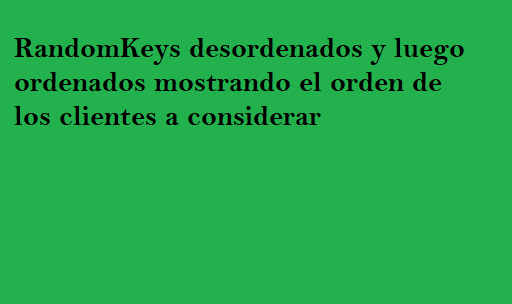
\includegraphics[width=14cm]{RandomKeysOrdenando}
	\label{fig:RandomKeysOrdenando}
\end{figure}

\subsection{Decodificador Simple}

El decodificador simple recibe como parámetro el vector de \textit{RandomKeys} y lo primero que hace es obtener los clientes ordenados como describimos anteriormente. Luego por cada vehículo, si el siguiente cliente se puede incluir en la ruta se incluye sino considera que la ruta esta completa y pasa al siguiente vehículo. Estos se puede ver en detalle en el pseudocódigo \ref{func:decodeSimple}. 

\bigskip

\begin{minipage}{\linewidth}
\begin{lstlisting} [caption={Función \textit{Decode} del decodificador simple.}, label={func:decodeSimple}]
public Solution Decode(List<RandomKey> randomKeys, ProblemInfo pi)
{
	var clients = GetOrderedClients(randomKeys);
	var vehicles = pi.GetVehicles();	
	var iv = 0;
	var ic = 0;	
	do
	{
		if(vehicles[iv].CanVisit(clients[ic]))
		{
			vehicles[iv].AddClient(clients[ic]);
			ic++;
		}
		else
		{
			iv++;			
		}
		
	} while(iv < vehicles.Length && ic < clients.Length)	
	var solution = pi.InstanceSolution(vehicles);
	return problem;
}
\end{lstlisting}
\end{minipage}

Un cliente $c_i$ se puede agregar a la ruta si al agregarlo, la ruta no supera su distancia máxima permitida. Sean $v$ vehículo, $d_{max}$ la distancia máxima de $v$, $d_{act}$ la distancia actual de la ruta de $v$, $n_f$ el nodo final de la ruta, $c_u$ el último cliente agregado a la ruta de $v$ y $c_i$ cliente que se intenta agregar a la ruta de $v$. Si aún no se insertaron clientes en la ruta, $c_u = n_i$ donde $n_i$ representa el nodo inicial de la ruta. Como podemos observar en el pseudocódigo \ref{func:decodeSimple}, creé un método llamado \textit{CanVisit}, que modela la fórmula \ref{eq:canVisit}. \textit{CanVisit} retorna \textit{true} cuando $c_i$ se puede agregar a la ruta y \textit{false} en caso contrario.

\bigskip

\begin{mycapequ}[!ht]
	\caption{El método \textit{CanVisit} retorna \textit{true} cuando la siguiente formula es válida:}
	\begin{equation} \label{eq:canVisit}
	d_{act}\, +\, distancia(c_u, c_i)\, +\, distancia(c_i, n_f)\, -\, distancia(c_u, n_f) \leq d_{max}
	\end{equation}
\end{mycapequ}

\bigskip

Una vez que terminé de implementar el decodificador simple, analicé el rendimiento de las soluciones generadas a partir de este decodificador. Hice este análisis para saber que tan buena sería la población inicial de mi algoritmo BRKGA cuando se utiliza el decodificador simple. Para realizar este análisis creé aleatoriamente 200 vectores de $RandomKeys$ que el decodificador simple convirtió en 200 soluciones válidas del problema. Sobre estas 200 soluciones calculé el beneficio máximo, promedio y mínimo, y sus índices de efectividad promedio y máximo. Esto se realizó para cada una de las seis instancias del benchmark seleccionadas anteriormente \ref{tab:instanciasDiversas}. Podemos observar los resultados en la tabla \ref{tab:resultadosDecoSimple}.

\bigskip

\begin{table}
\begin{center}
\begin{tabular}{ |c|c|c|c|c|c|c|c| } 
\hline
Instancia & N/V/D & $B_{min}$ & $B_{avg}$ & $B_{max}$ & $i_{eAvg}$ & $i_{eMax}$ & $Best$ \\
\hline
p2.2.k & 21/2/22.50 & 40 & 102 & 175 & 0.37 & 0.64 & 275 \\
p2.3.g & 21/3/10.70 & 45 & 83 & 140 & 0.57 & 0.97 & 145 \\
p3.4.p & 33/4/22.50 & 90 & 170 & 270 & 0.30 & 0.48 & 560 \\
p5.3.x & 66/3/40.00 & 195 & 295 & 405 & 0.19 & 0.26 & 1555 \\
p7.2.e & 102/2/50.00 & 8 & 39 & 98 & 0.13 & 0.34 & 290 \\
p7.4.t & 102/4/100.00 & 40 & 116 & 221 & 0.11 & 0.21 & 1077 \\
\hline
\end{tabular}
\end{center}
\caption{Resultados de las 200 soluciones generadas por el decodificar simple.}
\label{tab:resultadosDecoSimple}
\end{table}

En los resultados de la tabla \ref{tab:resultadosDecoSimple} vemos que para instancias pequeñas los resultados son mejores. En la instancia \textit{p2.3.g} una de las 200 soluciones quedo muy cercana a la mejor solucion conocida, obteniendo un $i_{eMax}=0.97$. Esta instancia tiene los mismos clientes que la instancia \textit{p2.2.k} pero como el $d_{max}$ de \textit{p2.3.g} es prácticamente la mitad que el de \textit{p2.2.k} luego la cantidad de combinaciones de rutas diferentes disminuye considerablemente. Es por eso que obtuve mejores resultados de \textit{p2.3.g}. Por otro lado podemos observar $i_{eAvg}$ disminuye a medida que la instancia tiene mayor número de clientes. Los peores resultados los obtuvo la instancia \textit{p7.4.t}, la instancia de mayor cantidad de clientes y mayor $d_{max}$.

\subsection{Características y debilidades del decodificador simple}

Este decodificador es simple y rápido, su orden de complejidad es de $O(\#clientes + \#veh\acute{\dotlessi}culos)$. En la práctica nunca se llega a visitar a todos los clientes ya que cambia de vehículo en cuanto encontró un cliente que no logró insertar en su ruta. Por lo tanto en la práctica nunca llega al orden de complejidad mencionado. Esto es una gran ventaja ya que en cada iteración del BRKGA se va a decodificar una cantidad $\#Poblaci\acute{o}n$ de veces. Luego una decodificación rápida nos permitirá mayor cantidad de generaciones.

\bigskip

Una característica menos relevante es el orden en que quedan los clientes asignados en los vehículos al ver el vector de \textit{RandomKeys}.  Sea $v$ el vector de clientes ordenados por un vector de \textit{RandomKeys}. Existen $m+1$ índices $i_0 = 0, i_1, i_2, .., i_m$ donde $m$ es la cantidad de vehículos y $0 \leq i_j \leq \#clientes$ tales que el vehículo $j$ incluye en su recorrido a todos los clientes del subvector $v[i_{j-1}, i_j-1]$. Luego todos los clientes en el subvector $v[i_m, v.Length - 1]$ son clientes no alcanzados por la solución. En otras palabras, los clientes quedan agrupados por vehículo cuando los vemos en el vector ordenado. Esto puede verse en la figura \ref{fig:DistribucionClientesDecoSimple}.

\begin{figure}[h]
	\caption{Posible distribución de clientes utilizando el decodificador simple para el vector de \textit{RandomKeys} de ejemplo. La primer ruta visita primero al cliente 6 y luego al 2. Como no pudo incluir al cliente 5, se cerró la ruta del primer vehículo y siguió con el próximo vehículo disponible. La segunda ruta visita al cliente 5 y luego al cliente 1. Como no pudo visitar al cliente 4 por la limitación de distancia, no intento agregar a los siguientes clientes.}
	\centering
	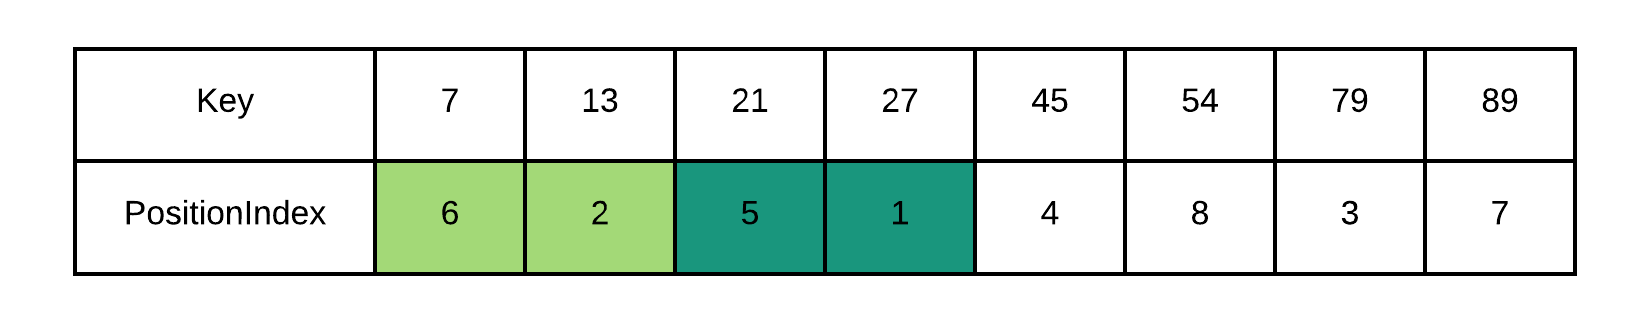
\includegraphics[width=14cm]{DistribucionClientesDecoSimple}
	\label{fig:DistribucionClientesDecoSimple}
\end{figure}

\bigskip

Un problema que tiene este decodificar es en la existencia de un cliente inalcanzable. Un cliente inalcanzable es aquel que no puede insertarse en una ruta aún cuando la ruta no contiene ningún otro cliente. En la función \ref{eq:inalcanzable} podemos distinguir cuando un cliente no se lo puede agregar en ninguna ruta.

\bigskip

\begin{mycapequ}[!ht]
	\caption{Función para evaluar si un cliente es inalcanzable.}
	\begin{equation} \label{eq:inalcanzable}
	distancia(n_i, c)\, +\, distancia(c, n_f)\, >\, d_{max}
	\end{equation}
\end{mycapequ}

\bigskip

Si utilizamos el decodificador simple y tenemos un cliente inalcanzable en el mapa, existe el escenario en el cual hay soluciones de la población donde todos los vehículos tienen sus rutas vacías. Supongamos que existe un cliente inalcanzable y que es el primer cliente que se intenta agregar en la ruta del primer vehículo. Como el cliente es inalcanzable no entra en la ruta, entonces se considera que el vehículo tiene la ruta completa y se pasa al siguiente vehículo dejando su ruta vacía. Esto se repite con todos los vehículos ya que tienen el mismo valor de $d_{max}$. La solución óptima a este problema es filtrar todos los clientes inalcanzables previo a la ejecución del BRKGA utilizando un método que modele la función \ref{eq:inalcanzable}. Haciendo esto no solo evitamos el escenario de rutas vacías, también reducimos el tamaño del problema antes de comenzar a resolverlo. 

\bigskip

Como el decodificador simple cambia de vehículo al primer intento fallido de expandir su ruta, las soluciones que genera tienen rutas muy pequeñas. Seguramente existen algunos clientes que podrían insertarse a la ruta del vehículo actual. Es por este motivo implementé el \textit{Decodificador Goloso}.


\subsection{Decodificador Goloso}

El decodificador goloso en principio funciona igual que el decodificador simple hasta que llega a un cliente que no puede agregar a la ruta de un vehículo determinado. En este caso, en vez de pasar a trabajar con el siguiente vehículo disponible, intenta agregar al siguiente cliente y así sucesivamente hasta que no hay más clientes con los cuales intentar agregar al vehículo actual. Después, al pasar al siguiente vehículo intenta con los clientes no asignados a los vehículos anteriores y siempre respetando el orden de los clientes asignado por el vector de \textit{RandomKeys}. Podemos ver en detalle como implementé el método \textit{Decode} del decodificador goloso en el pseudocódigo \ref{func:decodeGoloso}.  

\bigskip

\begin{minipage}{\linewidth}
\begin{lstlisting} [caption={Función \textit{Decode} del decodificador goloso. }, label={func:decodeGoloso}]
public Solution Decode(List<RandomKey> randomKeys, ProblemInfo pi)
{
	var clients = GetOrderedClients(randomKeys);
	var cIterator = new Iterator(clients);
	var vehicles = pi.GetVehicles();	
	var iv = 0;
	while(iv < vehicles.Length)
	{
		var currentClient = cIterator.Next;
		while(currentClient != null)
		{
			if(vehicles[iv].CanVisit(currentClient))
			{
				vehicles[iv].AddClient(currentClient);
				cIterator.Remove(currentClient);
			}
			currentClient = cIterator.Next;
		}
		cIterator.ToStartingPosition;
	}
	var solution = pi.InstanceSolution(vehicles);
	return problem;
}
\end{lstlisting}
\end{minipage}

\bigskip

Como podemos observar en el pseudocódigo \ref{func:decodeGoloso}, su complejidad es $0(\#clientes * \#veh\acute{\dotlessi}culos)$. El método \textit{Decode} es usado tantas veces a lo largo del BRKGA que este pequeño aumento en su complejidad algorítmica tiene un impacto visible en el tiempo de ejecución total. Por otro lado, utilizar el decodificador goloso mejora el beneficio de las soluciones generadas respecto de las soluciones generadas por el decodificador simple. Esa es la compensación que tenemos entre el decodificador simple y el goloso.

\bigskip

Otra característica que podemos mencionar sobre el decodificador goloso es que al observar el vector ordenado de \textit{RandomKeys}, ya no tenemos a los clientes de forma continua según su vehículo asignado como sucedía con el decodificador simple. Esto puede verse en la figura \ref{fig:DistribucionClientesDecoGoloso}.

\begin{figure}[h]
	\caption{Posible distribución de clientes utilizando el decodificador goloso para el vector de RandomKeys de ejemplo. La primer ruta visita a los clientes 6, 2 y por último al 8. El decodificador goloso no cerró la ruta del primer vehículo al no poder incluir al cliente 5, en cambio intenta con el resto de los clientes aún no visitados manteniendo el orden y logra insertar al cliente 8. De un modo similar, sucede con la segunda ruta al no poder incluir al cliente 4. Con el cliente 8 no lo intenta por que esta asignado a la primer ruta. Intenta con éxito insertar al cliente 3 y por último falla con el cliente 7. }
	\centering
	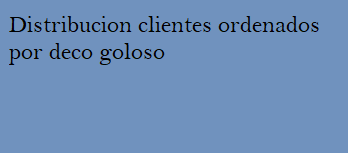
\includegraphics[width=14cm]{DistribucionClientesDecoGoloso}
	\label{fig:DistribucionClientesDecoGoloso}
\end{figure}

\bigskip

Le hice un análisis de rendimiento al decodificador goloso del mismo modo que lo hice con el decodificador simple. Generé otros 200 vectores de \textit{RandomKeys} para cada una de las mismas seis instancias de problemas y el decodificador goloso creó 200 soluciones válidas.

\begin{table}
\begin{center}
\begin{tabular}{ |c|c|c|c|c|c|c|c|c|c| } 
\hline
Instancia & N/V/D & $B_{min}$ & $B_{avg}$ & $B_{max}$ & $i_{eAvg}$ & $i_{eMax}$ & $Best$ \\
\hline
p2.2.k & 21/2/22.50 & 95 & 164 & 260 & 0.60 & 0.95 & 275 \\
p2.3.g & 21/3/10.70 & 95 & 122 & 140 & 0.84 & 0.97 & 145 \\
p3.4.p & 33/4/22.50 & 180 & 288 & 410 & 0.51 & 0.73 & 560 \\
p5.3.x & 66/3/40.00 & 305 & 412 & 525 & 0.26 & 0.34 & 1555 \\
p7.2.e & 102/2/50.00 & 31 & 96 & 163 & 0.33 & 0.56 & 290 \\
p7.4.t & 102/4/100.00 & 160 & 280 & 438 & 0.26 & 0.41 & 1077 \\
\hline
\end{tabular}
\end{center}
\caption{Resultados de las 200 soluciones generadas por el decodificar goloso.}
\label{tab:resultadosDecoGoloso}
\end{table}

\bigskip

Como podemos ver en la tabla \ref{tab:resultadosDecoGoloso}, todos los resultados promedio, mínimo y máximo mejoran considerablemente respecto de los resultados obtenidos con el decodificador simple (tabla \ref{tab:resultadosDecoSimple}). Tal es así, que tanto el $i_{eAvg}$ como el $i_{eMax}$ en algunos casos es mayor al doble de lo obtenido con en el decodificador simple. También se vuelve a observar como disminuye $i_{eAvg}$ a medida que crece el tamaño de la instancia del problema.

\section{Biased Random Key Genetic Algorithms}

En una primera instancia se implementa un BRKGA estándar. Dado una instancia de un problema, primero se genera la población inicial. Luego mientras no se cumpla la condición de parada, evolucionamos la población. Es decir se crea una nueva generación de soluciones a partir de la generación anterior como se explica en el capítulo~\ref{sec:brkga}. En el pseudocódigo \ref{func:RunBrkga} podemos ver un punto de vista macro del algoritmo BRKGA implementado.

\bigskip

\begin{minipage}{\linewidth}
\begin{lstlisting} [caption={Función \textit{RunBrkga}, vista macro de mi implementación.}, label={func:RunBrkga}]
public Solution RunBrkga(ProblemManager problemManager)
{
    var population = InitializePopulation();

    while (!StoppingRuleFulfilled(population))
        EvolvePopulation(population);

    return GetMostProfitableSolution(population);
}
\end{lstlisting}
\end{minipage}

\subsection{Configuración} \label{sec:config}

A modo de poder probar distintas configuraciones del BRKGA, creé el objeto \textit{Configuration} que instancia todas las variables que pueden impactan en el resultado final del BRKGA. Este objeto es esencial para ajustar mi implementación de una forma rápida y ordenada. Al centralizar todas las variables que podrían impactar en resultado final, gané mucho tiempo al probar variaciones de mi implementación. Además, al estar centralizada toda la información variable, se obtiene una lectura veloz del BRKGA que se esta probando. En otras palabras incrementé mi capacidad de monitoreo y control del desarrollo. El pseudocódigo \ref{func:config} muestra todas las propiedades configurables de mi desarrollo.

\bigskip

\begin{minipage}{\linewidth}
\begin{lstlisting} [caption={Objeto \textit{Configuration} donde se encuentran todas las variables importantes del BRKGA.}, label={func:config}]
public class Configuration
{
	public string Description { get; }
	public int MinIterations { get; set; }
	public int MinNoChanges { get; set; }
	public int PopulationSize { get; set; }
	public decimal ElitePercentage { get; set; }
	public decimal MutantPercentage { get; set; }
	public decimal EliteGenChance { get; set; }
	public List<ILocalSearch> LocalSearches { get; set; }
	public int ApplyLocalSearchesToTop { get; set; }
	public DecoderEnum DecoderType { get; set; }	
	private void SetDescription();
}
\end{lstlisting}
\end{minipage}

\bigskip

\subsection{Descripción y codificación de las propiedades configurables}\label{sec:descrCongif}

Como mencioné, uno de los beneficios de tener todas las variables configurables en un solo objeto es poder leer rápidamente que BRKGA estoy probando. A continuación explico las propiedades del objeto Configuración:

\begin{itemize}
  \item \textbf{Description}: Es una especie de hash descriptivo de la instancia del objeto \textit{Configuration}. Codifica los valores del resto de las propiedades utilizando su clave y valor.
  \item \textbf{MinIterations}: Clave \textbf{MI}. Valor entero utilizado en la función de corte. Cantidad mínima de generaciones que deben completar para cortar el BRKGA. 
  \item \textbf{MinNoChanges}: Clave \textbf{MNC}. Valor entero utilizado en la función de corte. Cantidad mínima de generaciones sin que aparezca una nueva mejor solución requerido para cortar el BRKGA.
  \item \textbf{PopulationSize}: Clave \textbf{PS}. Valor entero que denota el tamaño de la población.
  \item \textbf{ElitePercentage}: Clave \textbf{EP}. Valor decimal en el intervalo $(0, 1)$ que determina el tamaño de la población elite. Es un porcentaje de la población total.
  \item \textbf{MutantPercentage}: Clave \textbf{MP}. Valor decimal en el intervalo $(0, 1)$ que determina el tamaño mínimo de la población mutante. Es un porcentaje de la población total.
  \item \textbf{EliteGenChance}: Clave \textbf{EGC}. Valor decimal en el intervalo $(0, 1)$ que determina la probabilidad que tiene el alelo del padre de elite para transmitirse al individuo resultante del crossover.
  \item \textbf{LocalSearches}: Clave \textbf{LS}. Secuencia de algoritmos de búsquedas locales que se le aplicaran a la mejor solución de cada generación:
	\begin{itemize}
		\item \textbf{Swap}: Valor \textbf{S}.
		\item \textbf{Insert}: Valor \textbf{I}.
		\item \textbf{2-Opt}: Valor \textbf{O}.
		\item \textbf{Replace Simple}: Valor \textbf{Rs}.
		\item \textbf{Replace Multiple}: Valor \textbf{Rm}.
	\end{itemize}  
  \item \textbf{ApplyLocalSearchesToTop}: Clave \textbf{TOP}. Valor entero que denota la cantidad de soluciones a las cuales se les aplicaran las búsquedas locales.
  \item \textbf{DecoderType}: Clave \textbf{D}. Es una enumeración que determina el decodificador que se va a utilizar.
	\begin{itemize}
		\item \textbf{Simple}: Valor \textbf{S}.
		\item \textbf{Goloso}: Valor \textbf{G}.
	\end{itemize}  
\end{itemize}

\bigskip

El método \textit{SetDescription()} toma las tuplas de clave y valor del restos de las propiedades del objeto \textit{Configuración} y los concatena intercalados por un separador creando un \textit{string}. Podemos observar como lo hace en el pseudocódigo \ref{func:SetDescription}.

\bigskip

\begin{minipage}{\linewidth}
\begin{lstlisting} [caption={Método que instancia la propiedad \textit{Description}.}, label={func:SetDescription}]
public void SetDescription()
{ 
	var prop = Properties.Where(x => x.Name != "Description");
	var claveValores = prop.Select(p => p.Clave + "." + p.Valor);
	Description = string.Join(";", claveValores);
}
\end{lstlisting}
\end{minipage}

\bigskip

\begin{minipage}{\textwidth}
Entonces leyendo la propiedad \textit{Description} podemos ver como esta configurado el BRKGA. Por ejemplo si dice: 

\bigskip"MI.200;MNC.10;PS.100;EP.0,3;MP.0,1;EGC.0,7;LS.ISRsORm;TOP.2;D.G"

\begin{itemize}
  \item MinIterations: 200
  \item MinNoChanges: 10
  \item PopulationSize: 100
  \item ElitePercentage: 0,3
  \item MutantPercentage: 0,1
  \item EliteGenChance: 0,7
  \item LocalSearches: ISRsORm. Es la Secuencia: Insert, Swap, Replace Simple, 2-Opt y Replace Multiple.
  \item ApplyLocalSearchesToTop: 2
  \item DecoderType: Decodificador Goloso
\end{itemize}
\end{minipage}

\subsection{Inicialización de la Población}\label{subsec:InitializePopulation}

La población inicial se crea llamando al método \textit{AddMutants} que se explica en detalle más adelante. La inicialización de la población utiliza el mismo método que para crear soluciones mutantes ya que en ambos casos se requieren soluciones aleatorias. En el pseudocódigo \ref{func:InitializePopulation} vemos como el método \textit{InitializePopulation} devuelve las soluciones generadas por \textit{AddMutants}. El método \textit{AddMutants} toma como único parámetro el \textit{PopulationSize} que determina cuantos individuos deben ser creados.

\begin{minipage}{\linewidth}
\begin{lstlisting} [caption={Genereción de la población inicial.}, label={func:InitializePopulation}]
public Population InitializePopulation()
{ 
	var population = new Population();
	population.AddMutants(PopulationSize);
	return population;
}
\end{lstlisting}
\end{minipage}

\subsection{Condición de parada}

En una primera instancia de mi implementación la condición de parada era simple, el bucle terminaba cuando iteraba \textit{MinIterations} veces. Es decir que el bucle principal cortaba luego de evolucionar la población \textit{MinIterations} veces. Después de analizar varias ejecuciones noté que a veces la mejor solución de la población se había encontrado en las últimas evoluciones, por lo tanto agregue una condición de corte adicional: la mejor solución no debe haberse encontrado durante las últimas \textit{MinNoChanges} generaciones. Podemos ver ambas condiciones de parada en el pseudocódigo \ref{func:GenerateRandomKey}.

\bigskip

\begin{minipage}{\textwidth}
\begin{lstlisting} [caption={Condición de parada del BRKGA.}, label={func:GenerateRandomKey}]
public bool StoppingRuleFulfilled()
{ 
    return GenerationNum >= MinIterations && NoChanges();
}
private bool NoChanges()
{
	var currentProfit = CurrentBestSolution.GetProfit();
	return LastProfits.All(p => p == currentProfit);
}
\end{lstlisting}
\end{minipage}

El \textit{LastProfits} del pseudocódigo \ref{func:GenerateRandomKey}, es una cola de tamaño \textit{MinNoChanges} que contiene los beneficios de las mejores soluciones de las últimas generaciones. Si todos son iguales al beneficio de la mejor solución actual significa que no hubo cambios en las últimas \textit{MinNoChanges} generaciones.

\subsection{Evolución de la población}

Se toma la población y se ordenan sus individuos de forma descendente según su beneficio calculado con la función objetivo. Los mejores individuos pasan a ser parte de la población de elite y el resto de la población no-elite. El tamaño de la población de elite depende de la propiedad \textit{ElitePercentage} del objeto \textit{Configuration}. Luego se generan individuos mutantes, su cantidad es un porcentaje de la población total seteado por la propiedad \textit{MutantPercentage}. Finalmente se completa la nueva generación emparentando individuos de la población de elite con individuos de la población de no-elite. Los padres son elegidos al azar y el proceso de apareamiento se realiza como se describe en el la sección \ref{sec:brkga}. Durante el apareamiento, no es tan extraño que se genere una solución idéntica a otra ya existente en la población. De modo de no repetir soluciones, antes de insertar el individuo resultante se verifica que no exista otra solución idéntica en la nueva generación. De ser idéntica a otra solución, se genera una solución aleatoria del mismo modo que se generan los mutantes. En el pseudocódigo \ref{func:Evolve} podemos ver como evoluciona una población.

\bigskip

\begin{minipage}{\textwidth}
\begin{lstlisting} [caption={Evolución de la población.}, label={func:Evolve}]
public Population Evolve(Population population)
{
	var ordPopulation = population.GetOrderByMostProfitable();
	var elites = ordPopulation.Take(EliteSize);
	var nonElites = ordPopulation.Skip(EliteSize).Take(NonEliteSize);
	var evolvedPopulation = new Population(elites);
	evolvedPopulation.AddMutants(MutatansSize);
	while (evolvedPopulation.Size() < PopulationSize)
	{
		var anElite = GetRandomItem(elites);
		var aNoneElite = GetRandomItem(nonElites);
		var childSolution = Mate(anElite, aNoneElite);
		if (evolvedPopulation.Any(x => x.Equals(childSolution)))
			evolvedPopulation.AddMutants(1);
		else
			evolvedPopulation.Add(childSolution);
	}
	return evolvedPopulation;
}
\end{lstlisting}
\end{minipage}

\bigskip

Un proceso clave de la evolución es el \textit{crossover}. En el pseudocódigo \ref{func:Mate} observamos el proceso de apareamiento como lo describí en la sección \ref{sec:brkga}. Se crea un vector de \textit{RandomKeys} a partir de los vectores de \textit{RandomKeys} de un individuo elite y otro no-elite. Se determina que alelos recibirá el individuo resultante a partir de un decimal aleatorio en el intervalo [0, 1] y su comparación con la propiedad \textit{EliteGenChance}.

\bigskip

\begin{minipage}{\textwidth}
\begin{lstlisting} [caption={Crossover de dos individuos.}, label={func:Mate}]
private Solution Mate(Solution eliteP, Solution nonEliteP)
{
	var childRandomKeys = new List<RandomKey>();
	for (var index = 0; index < eliteP.RandomKeys.Count; index ++)
	{
		int key = 0;
		if(Random.NextDecimal(0, 1) >= EliteGenChance)
			key = eliteP.RandomKeys[index].Key;
		else
			key = nonEliteP.RandomKeys[index].Key;
		var randomKey = new RandomKey(key, index);
		childRandomKeys.Add(randomKey);
	}
	return Decoder.Decode(childRandomKeys, ProblemInfo);
}
\end{lstlisting}
\end{minipage}

\bigskip

Otro proceso muy importante de la evolución es la generación de los individuos mutantes. Cada uno es generado al azar a partir de un vector de \textit{RandomKeys}, del mismo modo que son generados los individuos de la población inicial como mencioné en \ref{subsec:InitializePopulation}. El pseudocódigo \ref{func:AddMutants} muestra como se crean los individuos mutante. El método \textit{AddMutants} toma como parámetro la cantidad de individuos que debe generar y por cada uno que debe generar crea un vector de \textit{RandomKeys}. Si la solución resultante del vector de \textit{RandomKeys} decodificado es igual a alguna de las soluciones existentes, deshace el vector de \textit{RandomKeys} y genera uno nuevo. En caso contrario agrega la solución a la población de soluciones.

\bigskip

\begin{minipage}{\textwidth}
\begin{lstlisting} [caption={Crossover de dos individuos.}, label={func:AddMutants}]
private void AddMutants(int amount)
{
	var solutions = new List<Solution>();
	for(var j = 0; j < amount; j++)
	{
		var randomKeys = new List<RandomKey>();
		for(i = 0; i < ProblemInfo.Clients.Length; i++)
		{
			var key = Random.Next(1000);
			var randomKey = new RandomKey(key, index);
			randomKeys.Add(randomKey)
		}		
		var solution = Decoder.Decode(randomKeys, ProblemInfo);
		if (Solutions.Any(x => x.Equals(solution)))
			j--;
		else
			Solutions.Add(solution);
	}	
}
\end{lstlisting}
\end{minipage}

\bigskip

Como mencioné en el proceso de evolución, mi implementación verifica que no se inserten soluciones duplicadas en la población. Verificar si dos soluciones son iguales tiene un costo temporal muy bajo en BRKGA. Como mencioné anteriormente el vector de \textit{RandomKeys} determina el orden de los clientes y para un orden de clientes determinado los decodificadores siempre generan la misma solución. Por lo tanto, para dos vectores de \textit{RandomKeys} que generen el mismo orden de clientes se obtienen la misma solución. Gracias a esto no es necesario comparar las rutas de dos soluciones para saber si son idénticas, es suficiente con comparar el orden en que se asignan sus clientes a las rutas. En el pseudocódigo \ref{func:GetHash} podemos ver como se crea el hash de una solución a partir de su vector de \textit{RandomKeys}. Para calcular el hash se ordena el vector de \textit{RandomKeys} por su campo \textit{Key}, después se toman los \textit{ClientId} y se los concatena con un símbolo separador. El hash se calcula una sola vez en el momento que se instancia la solución y su complejidad es de $O(clientes * log(clientes))$. Comparar dos hashs tiene una complejidad $O(1)$ ya que simplemente es comparar dos \textit{strings}. Por lo tanto verificar que la solución que se va a insertar no existe en la población tiene un complejidad de $O(poblaci\acute{o}n)$. En la figura \ref{fig:RandomKeysHash} podemos ver el ejemplo del hash de un vector de \textit{RandomKeys}.

\bigskip

\begin{figure}[h]
	\caption{Vector de \textit{RandomKeys} ordenado y su hash.}
	\centering
	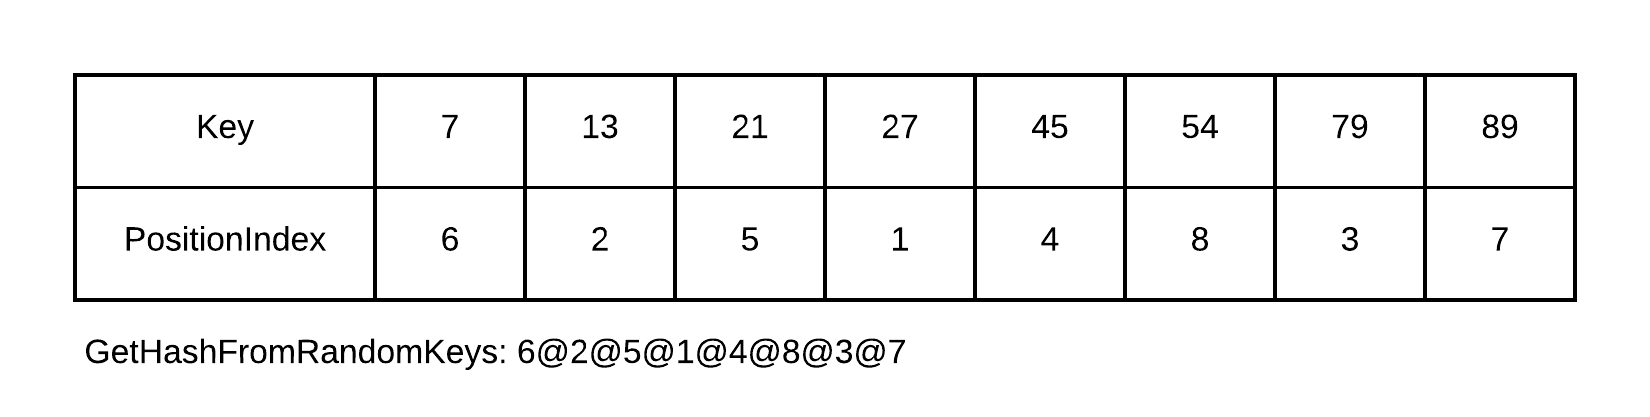
\includegraphics[width=14cm]{RandomKeysHash}
	\label{fig:RandomKeysHash}
\end{figure}

\bigskip

Decidí no reintentar el apareamiento entre los dos padres que generaron la solución repetida, porque consideré que la probabilidad de volver a generar nuevamente una solución existente es alta cuando ya sucedió una vez. Tomé la decisión de reemplazar por un mutante la solución repetida para optimizar el tiempo de ejecución del apareamiento y disminuir la cantidad de soluciones dentro de un mismo vecindario por generación.

\bigskip

\begin{minipage}{\textwidth}
\begin{lstlisting} [caption={Generación del hash de una solución.}, label={func:GetHash}]
private string pseudoHash;
public string GetHash()
{
	if (!string.IsNullOrEmpty(pseudoHash))
		return pseudoHash;
		
	var ork = RandomKeys.OrderBy(r => r.Key)
	pseudoHash = string.Join("@", ork.Select(k => k.ClientId));
	return pseudoHash;
}
\end{lstlisting}
\end{minipage}

\bigskip

En una primera instancia se insertaban los individuos sin verificar la existencia de un individuo idéntico en la población. Dada una población de soluciones no repetidas, la probabilidad de generar una solución existente al evolucionar la población es baja. Aún así, una vez que se genera una solución ya existente en la población, la probabilidad de que se genere otra copia más aumenta considerablemente. Esto se debe a que bajó la diversidad dentro de la población. A partir de la existencia de duplicados existe la posibilidad de utilizar padres idénticos. Si además la solución repetida se encuentra dentro del subconjunto de elite, la probabilidad aumenta aún más. Esto genera un efecto avalancha, donde la cantidad de individuos duplicados aumenta en cada evolución de la población. He llegado a obtener una población constituida de una única solución excepto por las soluciones mutantes. La existencia de duplicados reduce ampliamente la cantidad de soluciones diferentes exploradas, por ende reduce la frecuencia con la que una nueva mejor solución es generada. Además el algoritmo se vuelve más lento ya que repite cómputos en donde obtiene los mismos resultados. Lo que significa que el costo temporal total de validar unicidad en la inserción, que conlleva un orden de complejidad $O(poblaci\acute{o}n * poblaci\acute{o}nNoElite)$ por evolución, resulta muy bajo comparado con el costo de trabajar con múltiples soluciones duplicadas.

\subsection{Resultados de la primer versión}

Una vez que implementé el BRKGA puro (sin búsquedas locales), ejecuté la implementación diez veces para cada una de las seis instancias del benchmark previamente seleccionadas. Se pueden observar los resultados obtenidos en la tabla \ref{tab:resultadosBrkgaPuro}. Configuré el BRKGA de la siguiente manera: 

\bigskip

MI.250;MNC.10;PS.100;EP.0,3;MP.0,1;EGC.70;LS.;TOP.0;D.G (ver sección \ref{sec:descrCongif}).

\bigskip

\begin{table}
\begin{center}
\begin{tabular}{ |c|c|c|c|c|c|c|c|c|c|c| } 
\hline
Instancia & N/V/D & $T_{avg}$ & $B_{min}$ & $B_{avg}$ & $B_{max}$ & $i_{eAvg}$ & $i_{eMax}$ & $Best$ \\
\hline
p2.2.k & 21/2/22.50 & 2977 & 240 & 249 & 260 & 0.91 & 0.95 & 275 \\
p2.3.g & 21/3/10.70 & 1990 & 145 & 145 & 145 & 1.00 & 1.00 & 145 \\
p3.4.p & 33/4/22.50 & 6482 & 430 & 438 & 450 & 0.78 & 0.80 & 560 \\
p5.3.x & 66/3/40.00 & 17908 & 610 & 635 & 660 & 0.41 & 0.42 & 1555 \\
p7.2.e & 102/2/50.00 & 8753 & 204 & 217 & 246 & 0.75 & 0.85 & 290 \\
p7.4.t & 102/4/100.00 & 31532 & 458 & 481 & 513 & 0.45 & 0.48 & 1077 \\
\hline
\end{tabular}
\end{center}
\caption{Resultados de 10 ejecuciones del BRKGA puro sobre las seis instancias seleccionadas.}
\label{tab:resultadosBrkgaPuro}
\end{table}

\bigskip

De estos primeros resultados podemos ver que el BRKGA puro funciona muy bien para instancias de testeo pequeñas. Esto se refleja en la instancia \textit{p2.3.g} que siempre se llegó a la mejor solución posible y en \textit{p2.2.k} donde el $i_eAvg$ supera el 0.90. Luego a medida que incrementa el tamaño de la instancia, disminuye el $i_eAvg$. Es interesante ver como en la instancia \textit{p7.2.e} se obtuvieron resultados mucho mejores que aquellos obtenidos en la instancia \textit{p7.2.t} considerando que ambas pertenecen al \textit{set} siete. Es decir, tienen el mismo mapa de clientes y difieren en la cantidad de vehículos y el $d_{max}$ de los vehículos. Claramente al aumentar la cantidad de vehículos y el $d_{max}$ de los vehículos, aumenta considerablemente la cantidad de solucione posibles.

\bigskip

Con el objetivo de encontrar la mejor configuración general del BRKGA, tomé las dos instancias con menor $i_{eAvg}$ de la tabla \ref{tab:resultadosBrkgaPuro} y las utilice para probar distintas configuraciones. Los resultados de estos experimento se pueden observar en la tabla \ref{tab:resultadosBrkgaPuroCincoConfig}.

\bigskip

\begin{table}
\begin{center}
\begin{tabular}{ |c|c|c|c|c|c|c|c|c|c|c|c|} 
\hline
Instancia & N/V/D & Config & $T_{avg}$ & $B_{min}$ & $B_{avg}$ & $B_{max}$ & $i_{eAvg}$ & $i_{eMax}$ & $Best$ \\
\hline
p5.3.x & 66/3/40.00 & 1 & 60782 & 635 & 656 & 700 & 0.42 & 0.45 & 1555  \\
p5.3.x & 66/3/40.00 & 2 & 23363 & 620 & 636 & 660 & 0.41 & 0.42 & 1555  \\
p5.3.x & 66/3/40.00 & 3 & 22357 & 615 & 643 & 685 & 0.41 & 0.44 & 1555  \\
p5.3.x & 66/3/40.00 & 4 & 7311 & 475 & 498 & 555 & 0.32 & 0.36 & 1555  \\
p5.3.x & 66/3/40.00 & 5 & 54239 & 630 & 668 & 750 & 0.43 & 0.48 & 1555  \\
p7.4.t & 102/4/100.00 & 1 & 143760 & 472 & 506 & 542 & 0.47 & 0.50 & 1077  \\
p7.4.t & 102/4/100.00 & 2 & 42255 & 471 & 485 & 504 & 0.45 & 0.47 & 1077  \\
p7.4.t & 102/4/100.00 & 3 & 45952 & 463 & 488 & 542 & 0.45 & 0.50 & 1077  \\
p7.4.t & 102/4/100.00 & 4 & 11587 & 268 & 284 & 322 & 0.26 & 0.30 & 1077  \\
p7.4.t & 102/4/100.00 & 5 & 96642 & 478 & 491 & 509 & 0.46 & 0.47 & 1077  \\
\hline
\end{tabular}
\end{center}
\caption{Resultados de 10 ejecuciones del BRKGA puro sobre las seis instancias seleccionadas para cinco configuraciones generales diferentes.}
\label{tab:resultadosBrkgaPuroCincoConfig}
\end{table}

\bigskip

Configuraciones: 
\begin{itemize}
  \item \textbf{Config = 1}: MI.100;MNC.100;PS.500;EP.0,30;MP.0,05;EGC.70;LS.;TOP.0;D.G
  \item \textbf{Config = 2}: MI.150;MNC.30;PS.200;EP.0,25;MP.0,05;EGC.60;LS.;TOP.0;D.G 
  \item \textbf{Config = 3}: MI.150;MNC.70;PS.200;EP.0,30;MP.0,10;EGC.70;LS.;TOP.0;D.G
  \item \textbf{Config = 4}: MI.150;MNC.70;PS.200;EP.0,30;MP.0,10;EGC.70;LS.;TOP.0;D.S
  \item \textbf{Config = 5}: MI.250;MNC.50;PS.250;EP.0,15;MP.0,05;EGC.50;LS.;TOP.0;D.G 
\end{itemize}

\bigskip

Como síntesis de estos resultados observo que la configuración básica no tiene un fuerte impacto sobre el beneficio final de la ejecución. En el caso de la instancia \textit{p5.3.x}, el $i_{eAvg}$ siempre se encuentra en el intervalo [0.41,0.43] y en en \textit{p7.4.t} el intervalo es [0.45,0.47] siempre que se utiliza el decodificador simple. Para ambas instancias hay una configuración que es claramente peor y es la configuración \textbf{4} donde se utiliza el decodificar simple en vez del goloso. Por lo tanto en esta versión del BRKGA puro el decodificador tiene gran impacto en el resultado final. Lamentablemente el resto de las configuraciones impacta muy poco en el beneficio total cuando la instancia del problema es grande (Mínima cantidad de iteraciones, mínima cantidad de iteraciones sin cambios, tamaño de la población, población elite, etc). Si observamos los tiempos de ejecución, al comparar el $T_{avg}$ de la configuración \textbf{3} y \textbf{4} podemos ver que la configuración \textbf{3} es aproximadamente tres veces más lenta que la configuración \textbf{4} y solo difieren en el tipo de decodificador. Es muy claro que aunque el mejor beneficio obtenido con el decodificador simple es mucho menor, su tiempo de ejecución es mucho menor.

\bigskip

Como podemos ver en los resultados de la tabla \ref{tab:resultadosBrkgaPuro}, se pueden mejorar bastante los beneficios obtenidos y los tiempos de ejecución son bastante rápidos. Por lo tanto hay lugar para agregar mejoras al algoritmo sacrificando tiempo de ejecución en búsqueda de mejores resultados.

\bigskip

\section{Búsqueda Local}

Con el objetivo de optimizar los resultados obtenidos hasta el momento, implementé algunas búsquedas locales. La idea fue aplicar estas búsquedas a algunas de las mejores soluciones de cada generación. La cantidad de individuos a mejorar por generación es regida por el atributo \textit{ApplyLocalSearchesToTop} del objeto \textit{Configuration}. En caso de que a la solución ya se le hubiese aplicado las búsquedas en una generación anterior, se aplican a la siguiente mejor solución. Esto puede suceder ya que las mejores soluciones pertenecen al conjunto de elite y todos los individuos del conjunto de elite pasan directamente a la siguiente generación. Todas las búsquedas locales pueden modificar una solución ya sea para reducir su tiempo de recorrido o beneficio recolectado. La solución resultante de aplicar las búsquedas siempre es válida. Es decir, la solución resultante respeta la distancia máxima de la ruta de los vehículos y ningún cliente es visitado más de una vez. 

\subsection{Centro de Gravedad}

Para las búsquedas locales \textit{Insert} y \textit{Replace} se deben tomar una lista de clientes con algún orden. Este orden es importante ya que queremos empezar por las mejores opciones. El orden de clientes que se utiliza esta dado por su distancia al centro de gravedad (COG) de la ruta a la cual se le aplica el \textit{Insert} o el \textit{Replace}. Cuanto más cercano sea el cliente al COG de la ruta a optimizar, mayor prioridad tendrá el cliente. Implementé el cálculo del COG de la forma que lo describen Vansteenwegen et al. \cite{VansteenwegenSouffriauBergheOudheusden}. La coordenada del COG de una ruta se calcula como muestran las formulas \ref{eq:cogX} y \ref{eq:cogY}.

\begin{mycapequ}[!ht]
	\caption{Coordenada X del COG de una ruta.}
	\begin{equation} \label{eq:cogX}
	x_{cog} = (\sum_{\forall i \in ruta} x_i * B_i) / \sum_{\forall i \in ruta} B_i
	\end{equation}
\end{mycapequ}

\begin{mycapequ}[!ht]
	\caption{Coordenada Y del COG de una ruta.}
	\begin{equation} \label{eq:cogY}
	y_{cog} = (\sum_{\forall i \in ruta} y_i * B_i) / \sum_{\forall i \in ruta} B_i
	\end{equation}
\end{mycapequ}

\bigskip

Donde $x_i$ e $y_i$ son las coordenadas de un cliente de la ruta y $B_i$ es su beneficio. El cálculo del COG tiene una complejidad de $O(ruta.Length)$. Para no realizar cálculos innecesarios, el COG de una ruta solo se calcula cuando se necesita. Es decir, cuando la solución es seleccionada para ser mejorada. Se calcula una sola vez y cuando se modifica la ruta, se actualiza su COG.

\bigskip

Sea $r$ una ruta:

\begin{equation} \label{eq:cogNumDen}
r.x_{cog} =  \frac{\sum_{\forall i \in r.ruta} x_i * B_i}{\sum_{\forall i \in r.ruta} B_i}  = \frac{r.x_{cog.num}}{r.x_{cog.den}}
\end{equation}

\bigskip

Sea $r' = r.Remove(c_j)$ con $c_j$ cliente y $c_j \in r$:

\begin{equation} \label{eq:cogRemove}
r'.x_{cog} =  \frac{\sum_{\forall i \in r.ruta \wedge i \neq j} x_i * B_i}{\sum_{\forall i \in r.ruta \wedge i \neq j} B_i}  = \frac{r.x_{cog.num}-x_j*B_j}{r.x_{cog.den}-B_j}
\end{equation}

\bigskip

Sea $r'' = r.Add(c_k)$ con $c_k$ cliente y $c_k \notin r$:

\begin{equation} \label{eq:cogAdd}
r'.x_{cog} =  \frac{(\sum_{\forall i \in r.ruta} x_i * B_i) + x_k * B_k}{(\sum_{\forall i \in r.ruta} B_i) + B_k}  = \frac{r.x_{cog.num}+x_k*B_k}{r.x_{cog.den}+B_k}
\end{equation}

\bigskip

Cuando una ruta es modificada, el COG debe modificarse acorde. Si se elimina un cliente de una ruta, hay que remover del COG el impacto que tenía el cliente eliminado sobre el COG (Ídem cuando se inserta un cliente en la ruta). La actualizacion del COG puede implementarse con un complejidad de $O(1)$ si mantenemos los valores de $x_{cog.num}$ y $x_{cog.den}$ cuando calculamos el COG por primera vez como se observa en la formula \ref{eq:cogNumDen}. La formula \ref{eq:cogRemove} muestra como se actualiza el COG en $O(1)$ luego de remover un cliente utilizando los valores de $x_{cog.num}$ y $x_{cog.den}$. Ídem formula \ref{eq:cogAdd} para el caso en que se inserta un cliente.

\bigskip


\subsection{Swap}

El objetivo de esta búsqueda es encontrar e intercambiar clientes entre dos rutas distintas con el fin de disminuir la suma de las distancias recorridas de ambas rutas. Es decir, dados $v_a$ y $v_b$ vehículos y sus respectivas rutas $r_a$ y $r_b$, se puede realizar un \textit{Swap} entre sus rutas si existe un cliente $c_{a_i}$ en la ruta de $r_a$ y otro cliente $c_{b_j}$ en $r_b$ tal que agregando $c_{a_i}$ en alguna posición de $r_b$ y agregando $c_{b_j}$ en alguna posición de $r_a$ son válidas las formulas \ref{eq:swap1}, \ref{eq:swap2} y \ref{eq:swap3}.

\begin{equation}\label{eq:swap1}
r_a.Dist + r_b.Dist < r_a'.Dist + r_b'.Dist
\end{equation} 
\begin{equation}\label{eq:swap2}
r_a'.Dist \leq v'_a.d_{max}
\end{equation} 
\begin{equation}\label{eq:swap3}
r_b'.Dist \leq v'_b.d_{max}
\end{equation} 

\bigskip

En el pseudocódigo \ref{func:ApplyLocalSearchSwap} podemos ver que al aplicar esta búsqueda a una solución se ejecuta el método \textit{SwapDestinationsBetween} para todo par de rutas de la solución. Por lo tanto, este método será llamado $veh\acute{\dotlessi}culos * (veh\acute{\dotlessi}culos-1) / 2$ veces (la cantidad de combinaciones posibles de tomar dos elementos de un conjunto). El método \textit{SwapDestinationsBetween}, que podemos observar en el pseudocódigo \ref{func:SwapDestinationsBetween}, prueba intercambiar cada cliente de la ruta $a$ con cada cliente de la ruta $b$ y si efectivamente conviene hacer un \textit{Swap}, lo realiza. De modo de no estar cambiando múltiples veces a un mismo cliente entre dos rutas en una misma ejecución, cuando se cambia de ruta a un cliente se lo agrega en una lista de clientes prohibidos para intercambiar hasta que termine la ejecución actual del \textit{SwapDestinationsBetween}. Esta búsqueda local no mejora el beneficio total de una solución, lo que hace es disminuir la distancia recorrida de alguna ruta aumentando la probabilidad de insertar clientes no visitados.

\bigskip

\begin{minipage}{\textwidth}
\begin{lstlisting} [caption={Método \textit{ApplyLocalSearch} del \textit{Swap}.}, label={func:ApplyLocalSearchSwap}]
public bool ApplyLocalSearch(Solution solution)
{
	var changed = false;
	var combinations = GetCombinationsFor(solution.Vehicles.Count);
	foreach (var combination in combinations)
	{
		var v1 = solution.Vehicles[combination.Left];
		var v2 = solution.Vehicles[combination.Right];
		changed = changed || SwapDestinationsBetween(v1, v2);
	}
	return changed;
}
\end{lstlisting}
\end{minipage}

\begin{minipage}{\textwidth}
\begin{lstlisting} [caption={El método \textit{SwapDestinationsBetween}, prueba intercambiar todos los clientes entre dos rutas.}, label={func:SwapDestinationsBetween}]
public bool SwapDestinationsBetween(Vehicle v1, Vehicle v2)
{
	var changed = false;
	var v1Bans = new Dictionary<int, bool>();
	var v2Bans = new Dictionary<int, bool>();
	for (var i = 0; i < v1.Route.RouteLenght(); i++)
	{
		if(v1Bans.ContainsKey(i)) 
			continue;
		for (var j = 0; j < v2.Route.RouteLenght(); j++)
		{
			if (v2Bans.ContainsKey(j)) 
				continue;
			if (!Swaps(i, j, ref leftRoute, ref rightRoute)) 
				continue;
			changed = true;
			v1Bans.Add(i, true);
			v2Bans.Add(j, true);
			break; // Para que cambie i
		}
	}
	return changed;
}
\end{lstlisting}
\end{minipage}

\bigskip

El orden de complejidad del método \textit{ApplyLocalSearch} de la clase \textit{SwapHeuristic} es:

\begin{equation*}
O((n * (n-1) / 2 ) * clientes/n * clientes/n) \approx O(clientes^2/2)
\end{equation*}

\subsection{Insert}

El objetivo de esta búsqueda local es encontrar una posición en alguna ruta para un cliente no visitado sin sobrepasar el limite de distancia máxima de la ruta. Básicamente para cada vehículo y cada cliente no visitado se busca en que posición se debe insertar el cliente de forma tal que minimice el incremento de distancia recorrida. Si la distancia resultante es menor a la distancia máxima del vehículo, se inserta al cliente en tal posición. En caso contrario, no se inserta y se prueba con el siguiente cliente no visitado. El orden en que se toman los clientes no visitados es según su distancia al COG de la ruta a optimizar, de forma ascendente.

\begin{minipage}{\textwidth}
\begin{lstlisting} [caption={Método \textit{ApplyLocalSearch} del \textit{Insert}.}, label={func:ApplyLocalSearchInsert}]
public bool ApplyLocalSearch(Solution solution)
{
	var changed = false;	
	var uClients = solution.GetUnvistedClients;	
	var vehicles = solution.Vehicles;
	foreach (var vehicle in vehicles)
	{
		vehicle.Route.ActivateCog();
		uClients = uClients.OrderBy(x => vehicle.DistanceToCog(x));	
		for (var index = 0; index < uClients.Count; index++)
		{
			var res = AnalizeInsert(solution, vehicle, uClients[index]);
			if (res.CanBeInserted)
			{
				vehicle.AddDestinationAt(uClients[index], res.BestPosition);
				uClients.Remove(uClients[index]);
				changed = true;
			}
		}
	}
	return changed;
}
\end{lstlisting}
\end{minipage}

\bigskip

Como vemos en el pseudocódigo \ref{func:ApplyLocalSearchInsert} al empezar la ejecución del \textit{Insert}, lo primero que hace es activar el COG. Hasta el momento no había sido calculado para evitar cálculos innecesarios. Después de activar el COG, por cada cliente no visitado hasta el momento se analiza el \textit{insert}. El método \textit{AnalizeInsert} devuelve un objeto con dos propiedades que contienen la información necesaria para saber si se puede hacer el \textit{Insert} y donde. El objeto tiene una propiedad de tipo \textit{bool} que dice si el cliente puede ser insertado en el vehículo consultado. La otra propiedad dice cual es la mejor posición para insertar el cliente. Si el cliente es insertado en la ruta, se actualiza el COG de la ruta y se remueve el cliente de la lista de no visitados. El orden de complejidad del método \textit{ApplyLocalSearch} del \textit{Insert} es: 

\begin{equation*}
0(veh\acute{\dotlessi}culos * clientesNoVisitados * mediaClientesEnRuta)
\end{equation*}

\subsection{2-Opt}

El algoritmo \textit{2-Opt} es un algoritmo simple de búsqueda local propuesto por Croes \cite{Croes}. El objetivo es buscar un orden alternativo de los clientes visitados dentro de una misma ruta, de modo que disminuya la distancia recorrida por el vehículo. Es decir, un intercambio de posiciones entre dos clientes dentro de una misma ruta. Como podemos observar en el pseudocódigo \ref{func:ApplyLocalSearchInsert} se aplica el método \textit{Do2OptSwap} a cada vehículo de la solución.

\begin{minipage}{\textwidth}
\begin{lstlisting} [caption={Método \textit{ApplyLocalSearch} del \textit{Insert}.}, label={func:ApplyLocalSearchOptSwap}]
public bool ApplyLocalSearch(Solution solution)
{
	var index = 0;
	var changed = false;	
	var vehicles = solution.Vehicles;	
	while (index < vehicles.Count)
	{
		var currentDistance = vehicles[index].Route.GetDistance();
		changed = changed || Do2OptSwap(vehicles[index]);
		index++;
	}
	return changed;
}
\end{lstlisting}
\end{minipage}

\bigskip

El método \textit{Do2OptSwap} primero obtiene una lista de las todas las posibles cambios que se pueden hacer dentro de una ruta. Después por cada combinación intenta hacer un intercambio de posiciones dentro de la ruta. El intercambio se realiza solo si al hacerlo la distancia recorrida disminuye. Si en efecto se realiza el reemplazo, el bucle vuelve a empezar desde el principio debido a que el cambio puede generar nuevos reemplazos. Como el reemplazo solo sucede cuando la distancia resultante es estrictamente menor a la distancia original, el bucle siempre termina ya que la distancia del recorrido de la ruta no se puede reducir indefinidamente. El pseudocódigo \ref{func:OptSwap} muestra como implementé el \textit{2-Opt}.

\bigskip

\begin{minipage}{\textwidth}
\begin{lstlisting} [caption={Método \textit{ApplyLocalSearch} del \textit{Insert}.}, label={func:OptSwap}]
private bool Do2OptSwap(Vehicle vehicle)
{
	var changed = false;	
	var combinations = GetCombinationsFor(vehicle.Route);
	var index = 0;
	while (index < combinations.Count)
	{
		var pos1 = combinations[index].Postion1;
		var pos2 = combinations[index].Postion2;
		var swaped = vehicle.Route.SwapIfImproves(pos1, pos2);
		if (swaped)
		{
			changed = true;
			index = 0;
		}
		else
			index++;
	}
	return changed;
}
\end{lstlisting}
\end{minipage}


\begin{minipage}{\linewidth}
Este algoritmo tiene un orden de complejidad:

\begin{equation*}
\begin{split}
O(2Opt) &= O(veh\acute{\dotlessi}culos * mediaClientesEnRuta  * (mediaClientesEnRuta - 1) / 2) \\
            &= O(veh\acute{\dotlessi}culos * mediaClientesEnRuta^2 / 2)
\end{split}
\end{equation*}
\end{minipage}

\bigskip

\subsection{Replace Simple}

Esta búsqueda tiene como objetivo intercambiar un cliente no visitado por un cliente visitado de una ruta de forma tal que aumente el beneficio de la ruta. Del mismo modo que la búsqueda \textit{Insert}, los clientes no visitados se toman en orden según su distancia al COG de la ruta, empezando por los más cercanos. En el pseudocódigo \ref{func:ApplyLocalSearchReplaceSimple} vemos que se aplica el \textit{Replace Simple} a cada vehículo de la solución.

\bigskip

\begin{minipage}{\textwidth}
\begin{lstlisting} [caption={Método \textit{ApplyLocalSearch} del \textit{Replace}.}, label={func:ApplyLocalSearchReplaceSimple}]
public bool ApplyLocalSearch(Solution solution)
{	
	var vehicles = solution.Vehicles;
	var changed = false;	
	foreach (var vehicle in vehicles)
		changed = changed || Replace(solution, vehicle);
	return changed;
}
\end{lstlisting}
\end{minipage}

\bigskip

El \textit{Replace Simple} es similar al \textit{Insert}. El \textit{Replace Simple} comienza analizando cual es la mejor posición para insertar el cliente no visitado y lo inserta sin verificar que el $d_{max}$ del vehículo haya sido superado. En caso de que la solución siga siendo válida continua con el siguiente cliente del mismo modo que lo hace el \textit{Insert}. El \textit{Replace Simple} se diferencia del \textit{Insert} en el caso en que la solución pase a ser inválida. En tal caso, se debe remover algún cliente de forma tal que se vuelva a respetar la restricción de la distancia máxima, $d_{max}$. Por lo tanto el \textit{Replace Simple} busca un cliente de menor beneficio que el insertado, tal que al removerlo la ruta vuelva a tener una distancia recorrida menor a $d_{max}$. En caso de no encontrar ninguno se remueve el cliente que se había insertado en un principio. Si existen múltiples clientes candidatos a removerse, se elige el que minimice el recorrido de la ruta. Elegí priorizar distancia sobre beneficio en el caso de múltiples candidatos a remover. Tomé tal decisión por que también implementé otro reemplazo enfocado puramente en mejorar el beneficio de la ruta. De este modo los vecindarios explorados por ambas búsquedas de reemplazo contienen menor cantidad de soluciones en común. Llamé a esta búsqueda \textit{Replace Simple} por que tiene una complejidad algorítmica menor que el otro reemplazo y cuando se efectuá un reemplazo siempre se remueve a lo sumo un cliente visitado. Podemos ver el pseudocódigo del \textit{Replace Simple} en la figura \ref{func:ReplaceSimple}.

\bigskip

\begin{minipage}{\textwidth}
\begin{lstlisting} [caption={Método \textit{Replace}.}, label={func:ReplaceSimple}]
private bool Replace(Solution solution, Vehicle vehicle)
{
	var unvisited = solution.GetCurrentUnvistedDestination;
	var changed = false;
	vehicle.Route.ActivateCog();
	uClients = uClients.OrderBy(x => vehicle.DistanceToCog(x));	

	foreach (var client in uClients)
	{
		var res = AnalizeInsert(solution, vehicle, client);
		vehicle.AddDestinationAt(destination, res.BestInsertPosition);
		if (!res.CanBeInserted)
		{
			var justChanged = false;
			if(IsReplaceSimple())
				justChanged = RemoveWorst(vehicle, client);
			else
				justChanged = RemoveWorstGroup(vehicle, client);
			changed = changed || justChanged;
		}
		else
			changed = true;
	}
	return changed;
}
\end{lstlisting}
\end{minipage}

\bigskip

El método \textit{RemoveWorst} recibe como parámetros el vehículo que excedió $d_{max}$ y al cliente que se le insertó. El cliente que se insertó es el candidato que se removerá por defecto. Como podemos ver en el pseudocódigo \ref{func:RemoveWorst}, para cada cliente con menor beneficio que el beneficio del cliente insertado, se calcula la distancia resultante si se lo remueve. Finalmente se remueve aquel cliente que minimice la distancia de la ruta que en el peor de los casos es el mismo cliente que se insertó.

\bigskip

\begin{minipage}{\textwidth}
\begin{lstlisting} [caption={Selección del cliente a remover en el \textit{Replace Simple}.}, label={func:RemoveWorst}]
public bool RemoveWorst(Vehicle vehicle, Client inserted)
{
	var toRemove = inserted;
	var minDistance = vehicle.dMax;
	var route = vehicle.Route;
	foreach (var client in route)
	{
		if (client.Profit > inserted.Profit)
			continue;
		var distance = GetDistanceWithout(route, client);
		if (distance <= minDistance)
		{
			minDistance = distance;
			toRemove = client;
		}
	}
	vehicle.Route.RemoveClient(toRemove);
	return toRemove.Id != inserted.Id;
}
\end{lstlisting}
\end{minipage}

\bigskip

\begin{minipage}{\linewidth}
El \textit{Replace Simple} tiene un orden de complejidad:

\begin{equation*}
O(Replace Simple) = O(veh\acute{\dotlessi}culos * clientesNoVisitados * mediaClientesVisitados * 2)
\end{equation*}
\end{minipage}

\bigskip

\subsection{Replace Multiple}

El \textit{Replace Multiple} se diferencia del \textit{Replace Simple} de dos formas. La primer diferencia es que explora todos los reemplazos posibles incluso remover múltiples clientes visitados por un cliente no visitado. La segunda diferencia es que dentro de todas sus opciones para reemplazar, selecciona aquella que maximice el beneficio. En cambio el \textit{Replace Simple} cuando encuentra múltiples candidatos a remover elige aquel que minimice la distancia que recorre el vehículo. El \textit{Replace Multiple} tiene una complejidad algorítmica mayor al \textit{Replace Simple} ya que dentro de las opciones que explora incluye aquellas exploradas por el \textit{Replace Simple}. La segunda diferencia la agregue con el objetivo de diferenciar, aún más, las soluciones resultantes de aplicar uno u otra búsqueda.

\bigskip

En mi desarrollo el \textit{Replace Multiple} se diferencia del \textit{Replace Simple} durante la ejecución del método \textit{Replace} \ref{func:ReplaceSimple} descrito anteriormente. Si se está ejecutando un \textit{Replace Simple} se llama al método \textit{RemoveWorst} y si se está ejecutando el \textit{Replace Multiple} se llama al método \textit{RemoveWorstGroup}. Cuando comienza a ejecutarse el \textit{RemoveWorstGroup} \ref{func:RemoveWorstGroupOrDefault} lo primero que hace es armar una lista de los potenciales grupos de clientes a remover. Un grupo de clientes tiene el potencial de ser removido si la sumatoria de sus beneficios es menor al beneficio del cliente insertado. En el pseudocódigo \ref{func:RemoveWorstGroupOrDefault} un \textit{CandidateGroup} representa un potencial grupo de clientes a remover. Obtenida la lista de los grupos de clientes candidatos se filtran dejando solo aquellos grupos que al removerlos, la ruta resultante recorra una distancia menor a $d_{max}$. Si después del filtrado queda un solo grupo, se eliminan los clientes de tal grupo. Si hay varios grupos de clientes candidatos, se remueven de la ruta los clientes del grupo cuya sumatorio de beneficios sea menor. Si no queda ningún grupo, se elimina el cliente que se insertó.

\bigskip

\begin{minipage}{\textwidth}
\begin{lstlisting} [caption={Selección de los clientes a remover en el \textit{Replace Multiple}.}, label={func:RemoveWorstGroupOrDefault}]
public bool RemoveWorstGroup(Vehicle vehicle, Client inserted)
{
	var changed = false;
	var candidatesToRemove = new CandidateGroup(inserted);	
	var route = vehicle.Route;	
	var candidateGroups = new List<CandidateGroup>();
	candidateGroups = GetCandidateGroups(route, client); 	
	
	var bestOption = false;
	var valid = false;
	
	foreach(var candidateGroup in candidateGroups)
	{
		var distance = GetDistanceWithout(route, candidateGroup);
		valid = distance <= vehicle.dMax;
		bestOption = candidateGroup.Profit < candidatesToRemove.Profit;
		if(valid && bestOption)
		{
			candidatesToRemove = candidateGroup;
			changed = true;
		}
	}

	foreach (var client in candidatesToRemove.Clients)
		vehicle.Route.RemoveClient(client);

	return changed;
}
\end{lstlisting}
\end{minipage}

\bigskip

El pseudocódigo \ref{func:GetCandidateGroups} muestra como se obtienen los potenciales grupos de clientes a remover a partir del vehículo y el cliente insertado. Este método crea una lista con un tamaño máximo de $2^n-1$, siendo $n$ la cantidad de clientes en la ruta del vehículo. El peor caso sucede cuando el cliente insertado tiene un beneficio mayor a la sumatoria de beneficios de los clientes visitados. Por lo tanto el orden de complejidad de \textit{CandidateGroup} es de $O(2^{clientesVisitados})$ que es muy alto. De todos modos el peor escenario tiene una probabilidad muy baja de suceder, entonces el la práctica no es tan lento.

\bigskip

\begin{minipage}{\textwidth}
\begin{lstlisting} [caption={Método \textit{GetCandidateGroups}.}, label={func:GetCandidateGroups}]
public List<CandidateGroup> GetCandidateGroups(Vehicle v, Client c)
{
	var candidateGroups = new List<CandidateGroup>();
	var route = v.Route;
	for (var client in route)
	{
		if (client.Profit >= c.Profit)
			continue;		
		var newGroup = new CandidateGroup(client);
		foreach (var candidateGroup in candidateGroups)
			if (candidateGroup.Profit + client.Profit < inserted.Profit)
				candidateGroup.Add(client);
		candidateGroups.Add(newGroup);
	}
	return candidateGroups;
}
\end{lstlisting}
\end{minipage}

\bigskip

El \textit{Replace Multiple} mejoro considerablemente el $i_{eAvg}$ en instancias grandes ya que explora muchas más opciones que el \textit{Replace Simple} y prioriza el beneficio sobre la distancia. Esto lo hace sacrificando tiempo ya que su complejidad algorítmica es mayor a la del \textit{Replace Simple}. El \textit{Replace Multiple} tiene un orden de complejidad:

\begin{equation*}
O(Replace Multiple) = O(veh\acute{\dotlessi}culos * clientesNoVisitados * 2^{clientesVisitados})
\end{equation*}


\subsection{Encoder}

Agregar búsquedas locales entre generación de poblaciones conlleva un problema que debe resolverse. Al mejorar la solución se modifican sus rutas. Ahora bien, si no se actualizan los genes de una solución acorde a los cambios realizados por las búsquedas locales sus descendientes heredarán los genes de la solución no optimizada. Una vez que se optimiza una solución el vector de \textit{RandomKeys} debe ser actualizado de forma que sean validas la ecuaciones \ref{eq:reversibilidad} y \ref{eq:reversibilidad2}.

\bigskip

\begin{mycapequ}[!ht]
	\caption{Ecuaciones que deben ser válidas para que el \textit{crossover} sea correcto.}
	\begin{equation} \label{eq:reversibilidad}
	ApplyLocalSearch(s) = s'
	\end{equation}
	\begin{equation} \label{eq:reversibilidad2}
	s' = Decoder.Decode(s'.RandomKeys, ProblemInfo)
	\end{equation}
\end{mycapequ}

\bigskip

Como mencioné en la sección del Decodificador (ver sección \ref{sec:ordenDeco}), los clientes se ordenan de forma ascendente por la propiedad \textit{Key} del objeto \textit{RandomKey} asociado según la propiedad \textit{ClientId}. Por lo tanto el primer cliente con el que trabaja el decodificador, es el cliente con menor valor de \textit{Key}. Algo que no mencioné sobre la implementación de los decodificadores es que el primer vehículo por el que empieza es por el de menor \textit{Id} ya que los ordena por su \textit{Id} de forma ascendente. Los vehículos son indistinguibles al tener el mismo $d_{max}$ en el benchmark de instancias de problemas. De todos modos ahora debo respetar la decisión que tomé en el desarrollo de los decodificadores. Por lo tanto al primer cliente de la ruta del vehículo con menor \textit{Id} se le debe asociar el \textit{RandomKey} que tenga el menor \textit{Key}. Así, cuando el decodificador inicie, lo primero que hará es tomar este cliente e intentará adjudicárselo al primer vehículo, que justamente será el de menor \textit{Id}. Continuando con esta lógica el segundo cliente del mismo vehículo debe tener asignado el segundo \textit{RandomKey} de menor \textit{Key}. Y así sucesivamente, hasta tener mapeados todos los clientes del primer vehículo con su nuevo \textit{RandomKey}. Este proceso debe repetirse con los clientes del siguiente vehículo ordenados por \textit{Id} ascendentemente. Finalmente, quedarán sin \textit{RandomKey} asignado todos los clientes no visitados. En principio a estos clientes se les podría asignar cualquier \textit{RandomKey}. Aún así, en pos de disminuir los cambios genéticos sobre el individuo, se les asigna un \textit{RandomKey} tal que entre ellos mantengan el mismo orden que tenían antes de la mejora. Es decir, dentro de los clientes no visitados, el cliente que previamente tenía el \textit{RandomKey} con menor \textit{Key}, se le asigna el \textit{RandomKey} de menor \textit{Key} que queda disponible. 

\bigskip

En la figura \ref{fig:codificacionDeSolucionUno} podemos observar un vector de \textit{RandomKeys} ordenado por su campo \textit{Key}. Los \textit{ClientId} resaltados con color verde claro pertenecen al primer vehículo y los resaltados con verde oscura pertenecen al segundo vehículo. Debajo del vector de \textit{RandomKeys} podemos ver el hash de la solución y por último las rutas que fueron generadas por el decodificador goloso (los mismo clientes que estaban coloreados en el vector de \textit{RandomKeys}).

\bigskip

\begin{figure}[h]
	\caption{Dado un \textit{RandomKeys}, se obtiene un hash y una solución generada por el decodificador goloso.}
	\centering
	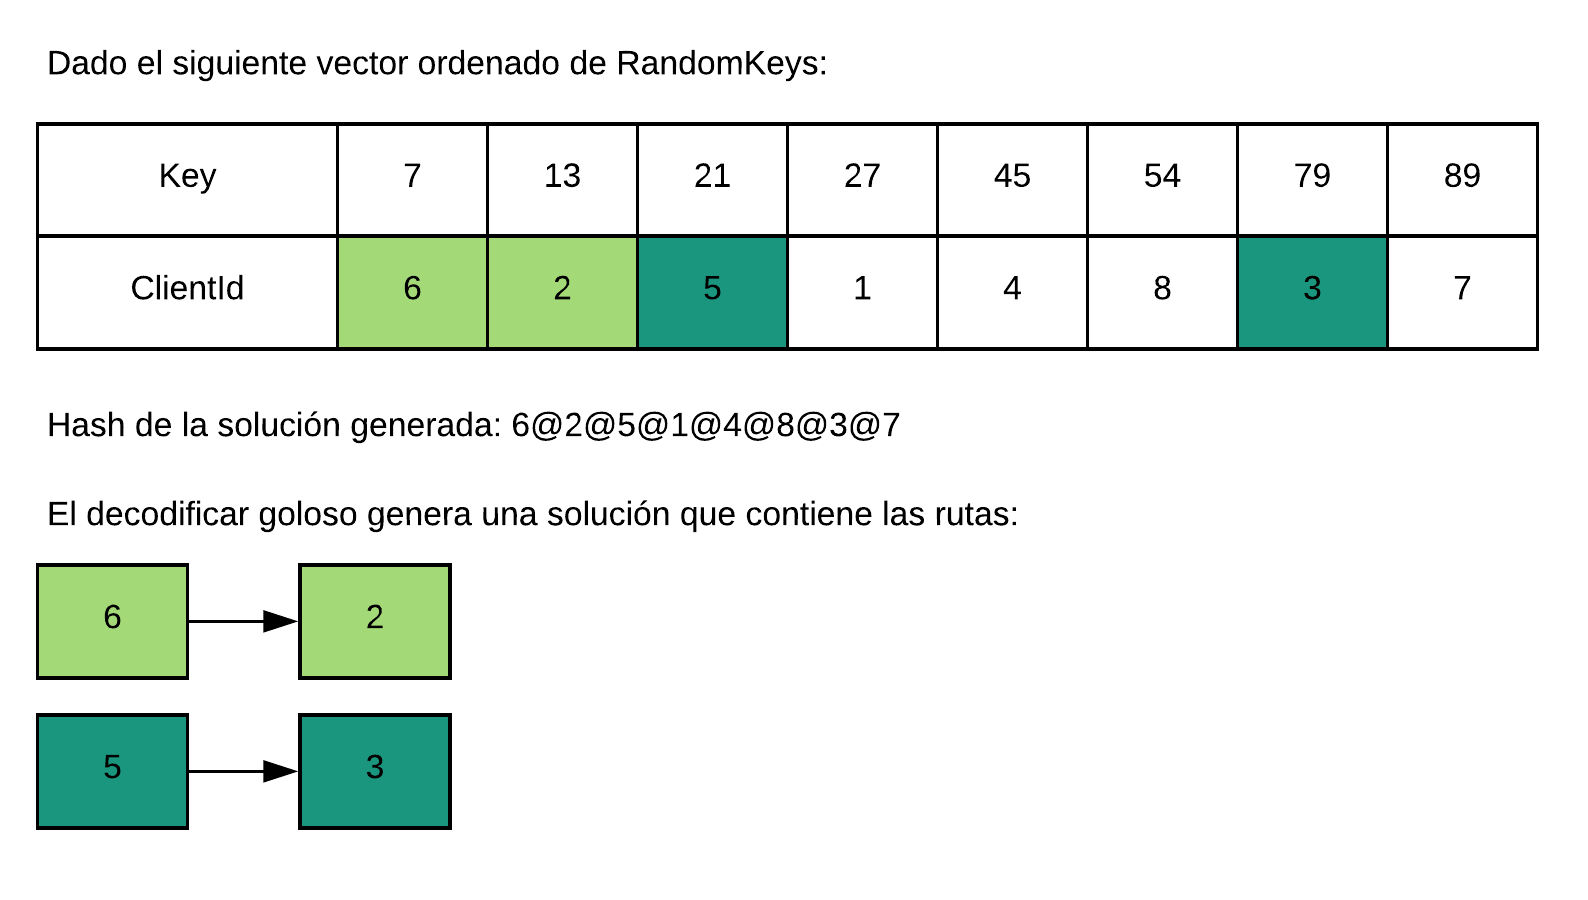
\includegraphics[width=14cm]{codificacionDeSolucionParteUno}
	\label{fig:codificacionDeSolucionUno}
\end{figure}

\bigskip

A la solución de la figura \ref{fig:codificacionDeSolucionUno} se le aplican algunas búsquedas locales y podemos ver los cambios en la figura \ref{fig:codificacionDeSolucionDos}. Ambas rutas se extienden con un nuevo cliente, la primer ruta incluso cambia el orden en que se visitan el cliente 2 y el 6. Debajo de las rutas vemos el vector de \textit{RandomKeys} ordenado por su campo \textit{Key} con los campos \textit{ClientId} actualizados de forma tal que al decodificar el vector de \textit{RandomKeys} genere la solución optimizada.

\bigskip

\begin{figure}[h]
    \caption{Se aplican búsquedas locales a la solución de la figura \ref{fig:codificacionDeSolucionUno}, después se actualiza el \textit{RandomKeys} y el hash de la solución. }
    \centering
    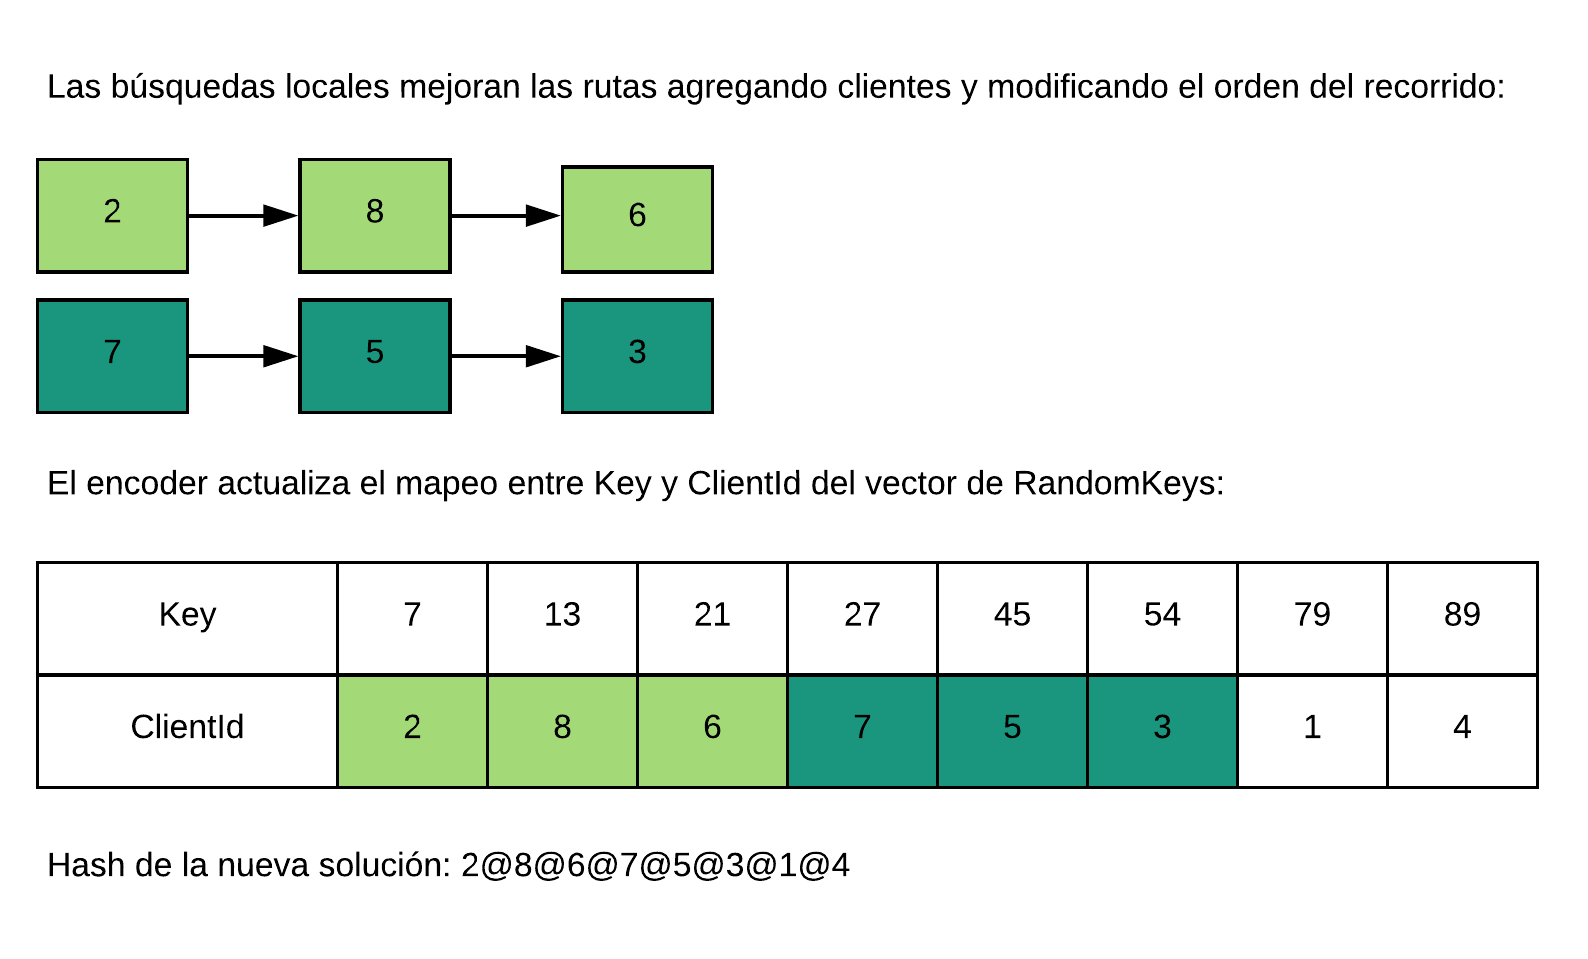
\includegraphics[width=14cm]{codificacionDeSolucionParteDos}
    \label{fig:codificacionDeSolucionDos}
\end{figure} 

Existe un escenario en donde al decodificar un \textit{RandomKeys} actualizado por el codificador no genere exactamente la misma solución que fue optimizada. Supongamos que tenemos el \textit{RandomKeys} de la figura \ref{fig:codificacionDeSolucionDos} que fue actualizado por el codificador luego de que la solución a la cual corresponde fuera optimizada por las búsquedas locales. Cuando el decodificador goloso le asigna el ClientId 6 al primer vehículo antes de cambiar de vehículo intentará asignar el resto de los clientes al primer vehículo. Lo que normalmente sucederá es que no logre insertar ninguno de los otros clientes, pero podría ser que alguno de los clientes pueda insertarse en el primer vehículo. De ser así existen dos opciones. La primera es que el cliente extra que se agregara a la primer ruta pertenezca a otro vehículo. En el ejemplo de la figura \ref{fig:codificacionDeSolucionDos} podría ser el caso los ClientId: 7, 5 o 3. Si sucede esto, el segundo vehículo tendría más tiempo disponible y menor beneficio. Si al segundo vehículo no se le inserta ningún cliente extra, el beneficio total de la solución se mantiene. En caso contrario algún cliente no visitado ahora tiene lugar en el segundo vehículo y el beneficio de la solución incremento. La segunda opcion es que el cliente extra insertado en el primer vehículo era un cliente no visitado. En el ejemplo de la figura \ref{fig:codificacionDeSolucionDos} podría ser el caso los ClientId: 1 o 4. Luego el segundo vehículo no se vería afectado. Lo que significa que el beneficio total de la solución aumento. Por lo tanto existen escenarios donde la ecuación \ref{eq:reversibilidad} no es válida pero el beneficio total de la solución resultante es igual o mayor a la que debería ser. Entonces no es un problema grave, además es un escenario poco factible ya que significaría que las búsquedas \textit{Insert}, \textit{Replace Simple} y \textit{Replace Multiple} no encontraron esta mejor solución que es vecina de la solución encontrada. De todos modos, opte por implementar unos delimitadores que agrega el codificador al actualizar el vector de \textit{RandomKeys} de forma tal que cuando los decodificadores pasan por uno de estos delimitadores son forzados a cambiar de vehículo. Esto asegura la validez de la ecuación \ref{eq:reversibilidad}. Podemos observar el pseudocódigo \ref{func:UpdateRandomKeys} que actualiza el vector de \textit{RandomKeys} luego de que la solución es optimizada por las búsquedas locales.

\bigskip

\begin{minipage}{\textwidth}
\begin{lstlisting} [caption={Método que actualiza el vector de \textit{RandomKeys}.}, label={func:UpdateRandomKeys}]
public static Solution UpdateRandomKeys(Solution s);
{
	var randomKeys = s.GetOrderedRandomKeys();
	// Todas las keys ordenadas ascendente
	var keys = randomKeys.Select(k => k.Key).ToList();
	var ClientIds = new List<int>();
	// Get ClientId from Visited Clients
	foreach (var r in s.Routes)
	{
		var d = r.GetDestinations();
		var rci = d.Select(d => d.ClientId);
		ClientIds.AddRange(rci);
	}
	// Get ClientId from Unvisited Clients
	var uClientIds = GetUnvisitedClientIds(randomKeys, newRoutes);
	ClientIds.AddRange(uClientIds);

	// Hay un break por cada cantidad de clientes en ruta 
	var breaks = new Queue(newRoutes.Select(r => r.ClientsCount));

	var newRandomKeys = new List<RandomKey>();
	var endRoute = false;
	var acumBreak = 0;
	for (var index = 0; index < keys.Count; index++)
	{
		if (breaks.Count > 0)
		{		
			endRoute = index + 1 == (int)breaks.Peek() + acumBreak;
			if (endRoute)
				acumBreak += (int)breaks.Dequeue();
		}		
		var randomKey = new RandomKey()
		{
			Key = keys[index],
			ClientId = ClientIdes[index],
			ForceVehicleChangeAfterThis = endRoute
		};
		newRandomKeys.Add(randomKey);
	}
	s.SetRandomKeys(newRandomKeys);
	return s;
}
\end{lstlisting}
\end{minipage}

Como se puede observar en los pseudocódigo de las búsquedas locales (\ref{func:ApplyLocalSearchSwap}, \ref{func:ApplyLocalSearchInsert}, \ref{func:ApplyLocalSearchOptSwap} y \ref{func:ApplyLocalSearchReplaceSimple}), todas implementan el método \textit{ApplyLocalSearch} que toma una solución y retorna un booleano que vale true si la solución fue modificada y false en caso contrario. Esto lo implementé así para poder ejecutar todas las búsquedas locales en una secuencia sin saber cual es el orden de la secuencia antes de la instanciación del BRKGA. De esta forma puedo setear la secuencia con el objeto \textit{Configuration} en el momento que se instancia el BRKGA. Gracias a esto pude probar las búsquedas locales en múltiples órdenes distintos. En el pseudocódigo \ref{func:ApplyLocalSearchesAll} podemos ver como se aplican las búsquedas según el orden en que se encuentran en la lista que toma de parámetro. Después de aplicar las búsquedas, si la solución fue modificada se actualiza el vector de \textit{RandomKeys}.

\begin{minipage}{\textwidth}
\begin{lstlisting} [caption={Aplicación de las búsquedas locales a una solución.}, label={func:ApplyLocalSearchesAll}]
public Solution ApplyLS(List<ILocalSearch> list, Solution solution)
{	
	var changed = false;
	foreach (var localSearch in list)
		changed = changed || localSearch.ApplyLocalSearch(solution);

	if(changed)
		solution = Encoder.UpdateRandomKeys (solution);
	
	return solution
}
\end{lstlisting}
\end{minipage}

\subsection{Orden de ejecución de las búsquedas locales}

Como mencioné previamente la lista de búsquedas locales se setea en el momento en que se instancia el BRKGA y las búsquedas se aplican en el orden en que se encuentran en la lista. Por ejemplo, si \textit{lista = (Swap, Insert, Replace Multiple)}, entonces primero se aplicará el \textit{Swap}, seguido del \textit{Insert} y finalmente el \textit{Replace Multiple}. La lista puede contener búsquedas repetidas, por ejemplo \textit{lista = (Swap, Insert, 2-Opt, Insert)}. El orden en que se ejecutan las búsquedas locales tiene un impacto fuerte sobre la solución final generada.

\bigskip

Con el objetivo de encontrar la mejor secuencia de búsquedas locales a aplicar, generé 7 configuraciones distintas para mi BRKGA que solo difieren en las listas de búsquedas locales. Para cada una de las 7 configuraciones ejecuté el BRKGA 25 veces sobre las dos instancias de problemas para las cuales había obtenido los peores resultados en el BRKGA puro. La configuración básica que comparten todas las configuraciones es la siguiente: 

\bigskip

MI.400;MNC.100;PS.150;EP.0,3;MP.0,1;EGC.0,70;TOP.2;DT.S.

\bigskip

Recordando los códigos de las búsquedas locales: 
\begin{itemize}
  \item \textbf{I}: Insert (Cliente no visitado)
  \item \textbf{Rs}: Replace Simple (Cliente no visitado por uno visitado)
  \item \textbf{Rm}: Replace Mutiple (Cliente no visitado por uno o varios visitado/s)
  \item \textbf{0}: 2-Opt (Swap dentro de una misma ruta)
  \item \textbf{S}: Swap (Swap entre dos rutas distintas)
\end{itemize}

\bigskip

\begin{table}
\begin{center}
\begin{tabular}{ |c|c|c|c|c|c|c|c|c|c|c| } 
\hline
Instancia & Search & $T_{avg}$ & $B_{min}$ & $B_{avg}$ & $B_{max}$ & $i_{eAvg}$ & $i_{eMax}$ & $Best$ \\
\hline
p5.3.x & IRmRsOS & 49397 & 1460 & 1485 & 1540 & 0.95 & 0.99 & 1555  \\
p5.3.x & ORsSIRm & 39576 & 1485 & 1509 & 1525 & 0.97 & 0.98 & 1555  \\
p5.3.x & SIORsSORm & 43556 & 1495 & 1512 & 1535 & 0.97 & 0.99 & 1555  \\
p5.3.x & SOIORsRmSORm & 49449 & 1505 & 1522 & 1545 & 0.98 & 0.99 & 1555  \\
p5.3.x & SOIRsRm & 36595 & 1500 & 1512 & 1525 & 0.97 & 0.98 & 1555  \\
p5.3.x & SOSIRsSORm & 40375 & 1505 & 1521 & 1535 & 0.98 & 0.99 & 1555  \\
p5.3.x & SRsOIRm & 43423 & 1480 & 1510 & 1535 & 0.97 & 0.99 & 1555  \\
p7.4.t & IRmRsOS & 81876 & 1004 & 1038 & 1064 & 0.96 & 0.99 & 1077  \\
p7.4.t & ORsSIRm & 86537 & 1024 & 1038 & 1063 & 0.96 & 0.99 & 1077  \\
p7.4.t & SIORsSORm & 91839 & 1033 & 1049 & 1077 & 0.97 & 1.00 & 1077  \\
p7.4.t & SOIORsRmSORm & 126705 & 1042 & 1055 & 1069 & 0.98 & 0.99 & 1077  \\
p7.4.t & SOIRsRm & 82889 & 1032 & 1047 & 1071 & 0.97 & 0.99 & 1077  \\
p7.4.t & SOSIRsSORm & 94731 & 1038 & 1055 & 1071 & 0.98 & 0.99 & 1077  \\
p7.4.t & SRsOIRm & 90306 & 1024 & 1042 & 1067 & 0.97 & 0.99 & 1077  \\
\hline
\end{tabular}
\end{center}
\caption{Resultados de aplicar distintas listas de búsquedas locales.}
\label{tab:resultadosListaLS}
\end{table}

\bigskip

En la tabla \ref{tab:resultadosListaLS}, se pueden observar los resultados de variar el orden en que se aplican las búsquedas locales. Claramente el peor orden de búsquedas locales es IRmRsOS (\textit{Insert}, \textit{Replace Multiple}, \textit{Replace Simple}, \textit{2-Opt}, \textit{Swap}). Las búsquedas \textit{Insert} y \textit{Replace} intentan agregar más clientes o intercambiar por clientes más rentables mejorando el beneficio de la ruta. En cambio las búsquedas \textit{2-Opt} y \textit{Swap} modifican la secuencia en que se visitan los clientes seleccionados con el objetivo de minimizar la distancia recorrida de una ruta. Al ejecutar primero las búsquedas que incrementan el beneficio y luego las que reducen la distancia recorrida, no se hace uso de la distancia disminuida por \textit{2-Opt} y \textit{Swap}.

\bigskip

Entre las otras 6 combinaciones aquellas con mejor resultados en sus 25 ejecuciones fueron SOSIRsSORm y SOIORsRmSORm. Ambas son las únicas que obtuvieron un $i_{eAvg}$ de 0.98 para las dos instancias. La configuración SIORsSORm llego a encontrar la mejor solución conocida para la instancia \textit{p7.4.t} pero su $i_{eAvg}$ es de 0.97. Decidí priorizar el valor del $i_{eAvg}$ sobre el valor del $i_{eMax}$ porque el $i_{eMax}$ no es estable, por lo tanto no garantiza buenos resultados. Entre las dos configuraciones con mejor $i_{eAvg}$ seleccioné SOSIRsSORm por que como se puede observar en la tabla \ref{tab:resultadosListaLS} tuvo un tiempo de ejecución promedio al menos un 20\% menor al de la configuración SOIORsRmSORm.

\bigskip

Por último, antes de calcular los resultados finales sobre todo el bechmark de problemas, hice una prueba de eficiencia entre los dos decodificadores ahora que el BRKGA tiene búsquedas locales. Para las mismas dos instancias de la tabla \ref{tab:resultadosListaLS}, ejecute 10 veces el BRKGA variando solamente los decodificadores utilizados. Para esta prueba utilicé la lista de búsquedas locales que mejores resultados obtuvo en el análisis previo: SOSIRsSORm.

\bigskip

\begin{table}
\begin{center}
\begin{tabular}{ |c|c|c|c|c|c|c|c|c|c|c| } 
\hline
Instancia & Deco & $T_{avg}$ & $B_{min}$ & $B_{avg}$ & $B_{max}$ & $i_{eAvg}$ & $i_{eMax}$ & $Best$ \\
\hline
p5.3.x & G & 93131 & 1515 & 1525 & 1545 & 0.98 & 0.99 & 1555  \\
p5.3.x & S & 50313 & 1515 & 1524 & 1535 & 0.98 & 0.99 & 1555  \\
p7.4.t & G & 198831 & 1043 & 1047 & 1051 & 0.97 & 0.98 & 1077  \\
p7.4.t & S & 119328 & 1041 & 1051 & 1059 & 0.98 & 0.98 & 1077  \\
\hline
\end{tabular}
\end{center}
\caption{Resultados de aplicar distintos decodificadores al BRKGA con búsquedas locales.}
\label{tab:testMe}
\end{table}

\bigskip

En la tabla \ref{tab:testMe} podemos observar los resultados obtenidos sobre las instancias \textit{p5.3.x} y \textit{p7.4.t} para el BRKGA con búsquedas locales modificando solamente los decodificadores. Los beneficios obtenidos son prácticamente iguales utilizando cualquiera de los decodificadores. Donde podemos ver diferencias en los resultados es la columna $T_{avg}$, el tiempo promedio de ejecución. El decodificador goloso demoró aproximadamente un 80\% más en ejecutarse que el decodificador simple. Es por este motivo que elegí el decodificador simple para mis resultados finales.

\bigskip

Con estas últimas pruebas tengo definido la configuración final para el BRKGA. Una última observación que quiero hacer es lo mucho que mejoraron los resultados en las instancias grandes luego de implementar las búsquedas locales. En la tabla \ref{tab:resultadosBrkgaPuro} la instancia \textit{p7.4.t} obtuvo un $i_{eAvg}$ de 0.45 mientras que en la tabla \label{tab:resultadosLSDecos} obtuvo un $i_{eAvg}$ de 0.98. Consideré que los resultados se encontraban en un nivel muy satisfactorio y decidí pasar a calcular los resultados finales sobre todo el benchmark de problemas.



